% local macros

\newcommand{\ccaption}[2]{
%\begin{center}
%\parbox{0.85\textwidth}{
%\caption[#1]{\small{{#2}}}
\caption[#1]{{{#2}}}
%}
%\end{center}
}

\providecommand{\lsim}
{\;\raisebox{-.3em}{$\stackrel{\displaystyle <}{\sim}$}\;}
\providecommand{\gsim}
{\;\raisebox{-.3em}{$\stackrel{\displaystyle >}{\sim}$}\;}

\section{Gluon-Fusion process\footnote{M. Grazzini, F. Petriello,
J. Qian, F. Stoeckli (eds.); J. Baglio, R. Boughezal and D. de Florian.}}
\label{ggFsection}

\subsection{Higgs-boson production in gluon--gluon fusion}


Gluon fusion through a heavy-quark loop~\cite{Georgi:1977gs} (see \Fref{fig:triangle}) is the main production mechanism of the Standard Model 
Higgs boson at hadron colliders.  When combined with the decay channels $\PH\to\PGg\PGg$, $\PH\to \PW\PW$, and $\PH\to \PZ\PZ$, this production
mechanism is one of the most important for Higgs-boson searches and studies over the entire mass
range, $100\UGeV \lsim \MH \lsim 1\UTeV$, to be investigated at the LHC.

\begin{figure}[hbt]
\begin{center}
\SetScale{0.8}
\begin{picture}(120,80)(0,0)
\Gluon(0,20)(50,20){-3}{5}
\Gluon(0,80)(50,80){3}{5}
\ArrowLine(50,20)(50,80)
\ArrowLine(50,80)(100,50)
\ArrowLine(100,50)(50,20)
\DashLine(100,50)(150,50){5}
\Vertex(50,20){2}
\Vertex(50,80){2}
\Vertex(100,50){2}
\put(124,37){$\PH$}
\put(17,37){$\Pt,\Pb$}
\put(-12,14){$\Pg$}
\put(-12,62){$\Pg$}
\end{picture}  \\
\caption{\label{fig:triangle} Feynman diagram
contributing to $\Pg\Pg\to\PH$ at lowest order.}
\end{center}
\end{figure}

The dynamics of the gluon-fusion mechanism is controlled by strong interactions. Detailed studies
of the effect of QCD radiative corrections are thus necessary to obtain accurate theoretical predictions.
In QCD perturbation theory, the leading order (LO) contribution \cite{Georgi:1977gs}
to the gluon-fusion cross section is proportional to $\alphas^2$, where $\alphas$ is the QCD coupling constant.  The 
main contribution arises from the top quark, due to its large Yukawa coupling to the Higgs boson.  The QCD radiative corrections to this 
process at next-to-leading order (NLO) have been known for some time, both in the large-$\Mt$ limit~\cite{Dawson:1991zj,Djouadi:1991tka} and maintaining the full top- and bottom-quark mass dependence~\cite{Graudenz:1992pv,Spira:1995rr}. They increase the 
LO cross section by about $80{-}100\%$ at the LHC.  The exact calculation is very well approximated by the
large-$\Mt$ limit. When the exact Born cross section with the full dependence on the mass of the top quark is used
to normalize the result, the difference between the exact and the approximated NLO
cross sections is only a few percent.  The next-to-next-to-leading order (NNLO) corrections have been computed only in this 
limit~\cite{Harlander:2000mg,Catani:2001ic,Harlander:2001is,Harlander:2002wh,Anastasiou:2002yz,Ravindran:2003um,Blumlein:2005im},
leading to an additional increase of the cross section of about 
$25\%$.
%\footnote{In the quantitative comments we always consider the range $100{-}300\UGeV$ for $7$ and $14\UTeV$}
The NNLO calculation has been consistently improved by resumming the soft-gluon contributions
up to NNLL \cite{Catani:2003zt}. The result leads to an additional
increase of the cross section of about $7{-}9\%$ ($6{-}7\%$) at
$\sqrt{s}=7$ $(14)\UTeV$.
The NNLL result is nicely confirmed by the evaluation of the leading soft contributions at N$^3$LO \cite{Moch:2005ky,Laenen:2005uz,Idilbi:2005ni,Ravindran:2005vv,Ravindran:2006cg}.

Recent years have seen further progress in the computation of radiative corrections and in the assessment
of their uncertainties. The accuracy of the large-$\Mt$ approximation at NNLO has been studied in
\Brefs{Marzani:2008az,Harlander:2009bw,Harlander:2009mq,Harlander:2009my,Pak:2009bx,Pak:2009dg}. These papers have definitely shown that if the Higgs 
boson is relatively light 
($\MH\lsim 300\UGeV$), the large-$\Mt$ approximation works extremely well,
to better than $1\%$. As discussed below, these results allow us to formulate accurate theoretical predictions where the top and bottom loops 
are treated exactly up to NLO, and the higher-order corrections to the top contribution
are treated in the large-$\Mt$ approximation~\cite{Anastasiou:2008tj}.

Considerable work has also been done in the evaluation of electroweak (EW) corrections.
Two-loop EW effects are now known \cite{Djouadi:1994ge,Aglietti:2004nj,Degrassi:2004mx,Actis:2008ts,Actis:2008ug}.  
They increase the cross section by a factor that strongly depends on the Higgs-boson mass, changing from 
$+5\%$ for $\MH=120$\UGeV\ to about $-2\%$ for $\MH=300$\UGeV\ \cite{Actis:2008ug}.
The main uncertainty in the EW analysis comes from the fact that it is not obvious how to combine them with the large QCD corrections.
In the {\it partial factorization} scheme of \Bref{Actis:2008ug}
the EW correction applies only to the LO result. In the {\em complete factorization} scheme, the EW correction instead multiplies the full 
QCD-corrected cross section.
Since QCD corrections are sizeable, this choice has a non-negligible
effect on the actual impact of EW corrections in the computation.
The computation of the dominant mixed QCD--EW effects due to light quarks~\cite{Anastasiou:2008tj},
performed using an effective-Lagrangian approach,
supports the complete factorization hypothesis, suggesting that
EW corrections become a multiplicative factor times the full QCD expansion.  This result should be interpreted carefully 
since the effective theory is strictly valid only when $\MH\muchless\MW$.  However, as discussed later, it is expected to be a good approximation to 
the exact result 
for Higgs-boson masses below several hundred \UGeV\ for the same reasons that the large-$\Mt$ limit furnishes a good approximation to the 
exact top-mass dependent calculation up to nearly $\MH = 1$\UTeV.  Very recently, EW effects for
Higgs production at finite transverse momentum \cite{Keung:2009bs,Brein:2010xj} 
have also been studied. Their effect is at the $1\%$ level or smaller.

In the following we present the results of three updated computations, based 
on the work presented in \Brefs{Anastasiou:2008tj,deFlorian:2009hc}
(see \Sref{se:ggfXS1}) and \Brefs{Baglio:2010um,Baglio:2010ae}
(see \Sref{se:ggfXS2}).%
\footnote{The central values of these cross-section predictions are in 
good mutual agreement, but the error assessment -- in particular
of theoretical errors that go beyond mere scale uncertainties --
is still under debate, leading to this splitting
of cross-section predictions into parts I and II.
It is worth noting that both calculations (ABPS and dFG) include the 
exact NLO mass dependence already. Also, the $\PQb$ mass parametric 
error should be accounted for by scale variations.
The combined numbers in the Summary, \Sref{se:summary}, are based
on the two predictions (ABPS and dFG) of the next section;
the inclusion of the BD analysis described in \Sref{se:ggfXS2},
with a common combination of all uncertainties, is in progress.}
These calculations use MSTW2008 NNLO parton distribution functions (PDFs)~\cite{Martin:2009iq}.

%\noindent{\bf Calculation by Anastasiou, Boughezal, Petriello and Stoeckli} (ABPS) \cite{Anastasiou:2008tj}
%\subsection{Calculations by Anastasiou/Boughezal/Petriello/Stoeckli and by de Florian/Grazzini}
\subsection{Cross-section predictions I}
\label{se:ggfXS1}

The following predictions are based on calculations by
Anastasiou/Boughezal/Petriello/Stoeckli and by de Florian/Grazzini. 

The calculation by Anastasiou, Boughezal, Petriello and Stoeckli (ABPS) \cite{Anastasiou:2008tj}
starts from the exact NLO cross section with full dependence on the top- and bottom-quark masses
and includes the NNLO top-quark contribution
in the large-$\Mt$ limit. The result includes EW contributions~\cite{Aglietti:2004nj,Degrassi:2004mx,Actis:2008ug,Actis:2008ts} according 
to~\Brefs{Actis:2008ug,Actis:2008ts}, evaluated in the complete factorization scheme.  Mixed QCD--EW contributions \cite{Anastasiou:2008tj} are 
also accounted for, together with some effects from EW corrections at finite transverse momentum~\cite{Keung:2009bs}. The effect of soft-gluon 
resummation is mimicked
by choosing
the central value of the renormalization and factorization scales
as $\mu_R=\mu_F=\MH/2$.
The latter choice is also motivated by an improved convergence of the fixed-order QCD perturbative expansion.

%\noindent{\bf Calculation by de Florian and Grazzini} (dFG) \cite{deFlorian:2009hc}

The calculation by de Florian and Grazzini (dFG)
is a slightly improved version on the calculation presented in \Bref{deFlorian:2009hc}.
The starting point is the exact NLO cross section with full dependence on
the top- and bottom-quark masses, computed with the program {\sc HIGLU} \cite{Graudenz:1992pv,Spira:1995rr}, on top of which the NLL resummation of soft-gluon contributions is included.
Then, the top-quark contribution is considered and the
NNLL+NNLO corrections \cite{Catani:2003zt} are consistently added in the large-$\Mt$ limit. The result is finally corrected for EW 
contributions~\cite{Aglietti:2004nj,Degrassi:2004mx,Actis:2008ug,Actis:2008ts} according to~\Brefs{Actis:2008ug,Actis:2008ts} in 
the complete factorization scheme. The central value of factorization and renormalization scales is chosen
to be $\mu_F=\mu_R=\MH$.  The results of this calculation are available through an online calculator \cite{calculator}.

\begin{figure}[htb]
\vspace{5pt}
\begin{center}
\begin{tabular}{cc}
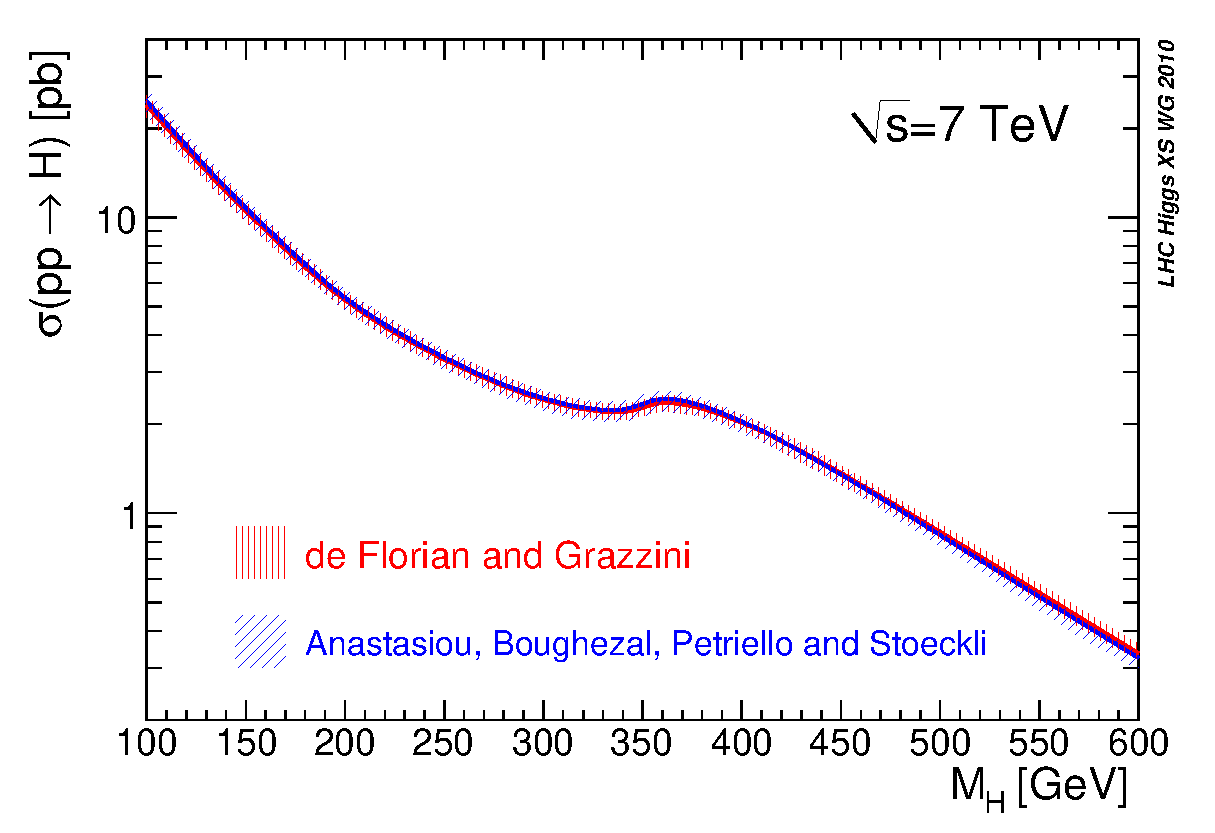
\includegraphics[width=.46\linewidth]{YRHXS_ggF/YRHXS_ggF_fig1} &
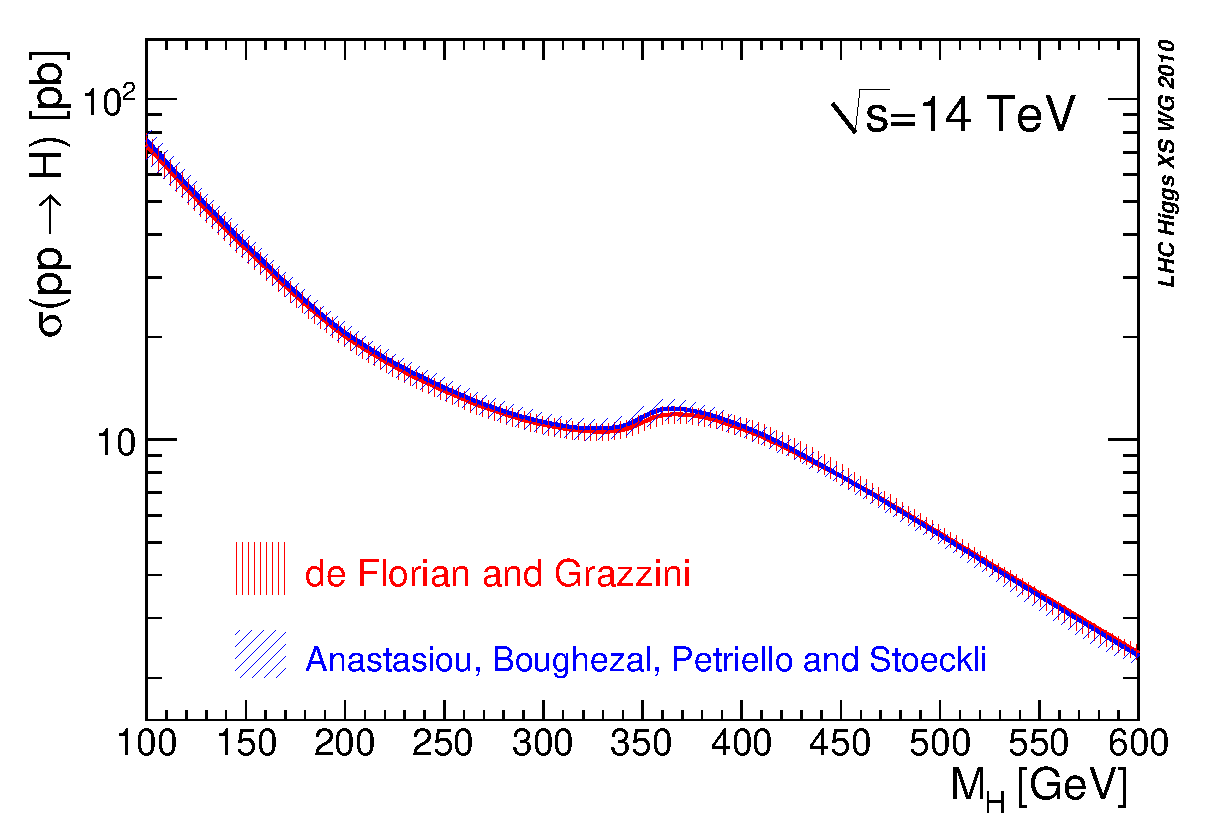
\includegraphics[width=.46\linewidth]{YRHXS_ggF/YRHXS_ggF_fig2}\\
\end{tabular}
\end{center}
\caption{Comparison of ABPS \cite{Anastasiou:2008tj} and dFG \cite{deFlorian:2009hc} results, including scale uncertainty bands.}
\label{fig:comp}
\end{figure}

The results of the dFG and ABPS calculations are reported in \Trefs{tab:dFG7},\ref{tab:dFG14} and \ref{tab:ABPS7},\ref{tab:ABPS14}, respectively.
For each Higgs-boson mass the corresponding cross section is reported.
We also quote three uncertainties: Scale uncertainty, PDF+$\alphas$ uncertainty,
and the latter uncertainty according to the PDF4LHC recipe, computed as discussed below.
In \Fref{fig:comp} we present a comparison of ABPS and dFG results, including scale uncertainties. We see that the results are perfectly 
consistent and show a very good agreement over a wide range of Higgs-boson masses.
At $\sqrt{s}=7$\UTeV\ the difference between ABPS and dFG central values ranges from $+3.5\%$ for $\MH=100$\UGeV\
to $-6\%$ for $\MH=1$\UTeV. In the range $\MH=115{-}300$\UGeV\ the difference ranges from $+3\%$ to $+1\%$.
At $\sqrt{s}=14$\UTeV\ the difference between ABPS and dFG central values ranges from $+3.7\%$ for $\MH=100$\UGeV\
to $-3\%$ for $\MH=1$\UTeV. In the range $\MH=115{-}300$\UGeV\ the difference ranges from $+3\%$ to $+2\%$.

%%%%%%%%%%%%%%%%%

\begin{table}
%\thisfloatpagestyle{empty}
%   \vspace{-\headsep}
   \begin{center}
   \ccaption{}{\label{tab:dFG7}{Results on $\Pp\Pp(\Pg\Pg)\to \PH+X$ cross sections with $\sqrt{s}=7$\UTeV\ based on dFG calculation, using MSTW2008 NNLO PDFs.}}
   \small
   \begin{tabular}{ccccc}
   \hline
   $\MH[\UGeVZ]$ & $\sigma[\UpbZ]$ & Scale [\%] & PDF+$\alphas$ [\%] & \small{PDF4LHC} [\%]\\
   \hline
$  90  $&$ 29.48 $& ${+ 8.2}   \;{- 8.7} $ & $ {+ 4.0}  \;{- 3.1} $ & ${+ 7.8}   \;{- 6.7} $ \\
$  95  $&$ 26.48 $& ${+ 8.0}   \;{- 8.6} $ & $ {+ 4.0}  \;{- 3.0} $ & ${+ 7.8}   \;{- 6.7} $ \\
$ 100  $&$ 23.97 $& ${+ 7.8}   \;{- 8.4} $ & $ {+ 4.0}  \;{- 3.0} $ & ${+ 7.7}   \;{- 6.8} $ \\
$ 105  $&$ 21.74 $& ${+ 7.7}   \;{- 8.3} $ & $ {+ 4.0}  \;{- 3.0} $ & ${+ 7.7}   \;{- 6.9} $ \\
$ 110  $&$ 19.81 $& $ {+ 7.5}  \;{- 8.1} $ & $ {+ 4.0}  \;{- 3.0} $ & $ {+ 7.7}  \;{- 6.9} $ \\
$ 115  $&$ 18.12 $& $ {+ 7.4}  \;{- 8.0} $ & $ {+ 4.0}  \;{- 3.0} $ & $ {+ 7.7}  \;{- 7.0} $ \\
$ 120  $&$ 16.63 $& $ {+ 7.2}  \;{- 7.9} $ & $ {+ 4.0}  \;{- 3.0} $ & $ {+ 7.6}  \;{- 7.0} $ \\
$ 125  $&$ 15.31 $& $ {+ 7.1}  \;{- 7.8} $ & $ {+ 4.0}  \;{- 3.1} $ & $ {+ 7.6}  \;{- 7.1} $ \\
$ 130  $&$ 14.13 $& $ {+ 7.0}  \;{- 7.7} $ & $ {+ 4.0}  \;{- 3.1} $ & $ {+ 7.6}  \;{- 7.2} $ \\
$ 135  $&$ 13.08 $& $ {+ 6.9}  \;{- 7.6} $ & $ {+ 3.9}  \;{- 3.1} $ & $ {+ 7.6}  \;{- 7.3} $ \\
$ 140  $&$ 12.14 $& $ {+ 6.8}  \;{- 7.5} $ & $ {+ 3.9}  \;{- 3.1} $ & $ {+ 7.6}  \;{- 7.3} $ \\
$ 145  $&$ 11.29 $& $ {+ 6.7}  \;{- 7.5} $ & $ {+ 3.9}  \;{- 3.1} $ & $ {+ 7.6}  \;{- 7.4} $ \\
$ 150  $&$ 10.52 $& $ {+ 6.6}  \;{- 7.4} $ & $ {+ 3.9}  \;{- 3.1} $ & $ {+ 7.6}  \;{- 7.5} $ \\
$ 155  $&$  9.80 $& $ {+ 6.5}  \;{- 7.3} $ & $ {+ 3.9}  \;{- 3.1} $ & $ {+ 7.5}  \;{- 7.5} $ \\
$ 160  $&$  9.08 $& $ {+ 6.4}  \;{- 7.2} $ & $ {+ 3.9}  \;{- 3.1} $ & $ {+ 7.5}  \;{- 7.6} $ \\
$ 165  $&$  8.35 $& $ {+ 6.4}  \;{- 7.2} $ & $ {+ 3.9}  \;{- 3.2} $ & $ {+ 7.5}  \;{- 7.7} $ \\
$ 170  $&$  7.76 $& $ {+ 6.3}  \;{- 7.1} $ & $ {+ 3.9}  \;{- 3.2} $ & $ {+ 7.5}  \;{- 7.8} $ \\
$ 175  $&$  7.24 $& $ {+ 6.2}  \;{- 7.0} $ & $ {+ 3.9}  \;{- 3.2} $ & $ {+ 7.5}  \;{- 7.8} $ \\
$ 180  $&$  6.76 $& $ {+ 6.2}  \;{- 7.0} $ & $ {+ 3.9}  \;{- 3.2} $ & $ {+ 7.5}  \;{- 7.8} $ \\
$ 185  $&$  6.32 $& $ {+ 6.1}  \;{- 6.9} $ & $ {+ 3.9}  \;{- 3.2} $ & $ {+ 7.5}  \;{- 7.8} $ \\
$ 190  $&$  5.92 $& $ {+ 6.1}  \;{- 6.9} $ & $ {+ 3.9}  \;{- 3.3} $ & $ {+ 7.5}  \;{- 7.8} $ \\
$ 195  $&$  5.57 $& $ {+ 6.1}  \;{- 6.8} $ & $ {+ 4.0}  \;{- 3.3} $ & $ {+ 7.5}  \;{- 7.8} $ \\
$ 200  $&$  5.27 $& $ {+ 6.0}  \;{- 6.8} $ & $ {+ 4.0}  \;{- 3.3} $ & $ {+ 7.6}  \;{- 7.8} $ \\
$ 210  $&$  4.74 $& $ {+ 6.0}  \;{- 6.7} $ & $ {+ 4.0}  \;{- 3.4} $ & $ {+ 7.5}  \;{- 7.9} $ \\
$ 220  $&$  4.29 $& $ {+ 6.5}  \;{- 6.6} $ & $ {+ 4.0}  \;{- 3.4} $ & $ {+ 7.6}  \;{- 7.9} $ \\
$ 230  $&$  3.92 $& $ {+ 5.9}  \;{- 6.5} $ & $ {+ 4.0}  \;{- 3.4} $ & $ {+ 7.7}  \;{- 8.0} $ \\
$ 240  $&$  3.59 $& $ {+ 5.9}  \;{- 6.4} $ & $ {+ 4.0}  \;{- 3.5} $ & $ {+ 7.7}  \;{- 8.0} $ \\
$ 250  $&$  3.32 $& $ {+ 5.8}  \;{- 6.3} $ & $ {+ 4.1}  \;{- 3.5} $ & $ {+ 7.8}  \;{- 8.1} $ \\
$ 260  $&$  3.08 $& $ {+ 5.8}  \;{- 6.3} $ & $ {+ 4.1}  \;{- 3.6} $ & $ {+ 7.8}  \;{- 8.1} $ \\
$ 270  $&$  2.87 $& $ {+ 5.8}  \;{- 6.2} $ & $ {+ 4.1}  \;{- 3.6} $ & $ {+ 7.9}  \;{- 8.1} $ \\
$ 280  $&$  2.70 $& $ {+ 5.8}  \;{- 6.1} $ & $ {+ 4.2}  \;{- 3.7} $ & $ {+ 7.9}  \;{- 8.2} $ \\
$ 290  $&$  2.55 $& $ {+ 5.8}  \;{- 6.1} $ & $ {+ 4.2}  \;{- 3.7} $ & $ {+ 8.0}  \;{- 8.3} $ \\
$ 300  $&$  2.42 $& $ {+ 5.8}  \;{- 6.0} $ & $ {+ 4.2}  \;{- 3.8} $ & $ {+ 8.0}  \;{- 8.3} $ \\
$ 320  $&$  2.25 $& $ {+ 5.8}  \;{- 6.0} $ & $ {+ 4.3}  \;{- 3.9} $ & $ {+ 8.2}  \;{- 8.4} $ \\
$ 340  $&$  2.20 $& $ {+ 5.8}  \;{- 5.9} $ & $ {+ 4.4}  \;{- 4.0} $ & $ {+ 8.3}  \;{- 8.4} $ \\
$ 360  $&$  2.36 $& $ {+ 5.8}  \;{- 5.9} $ & $ {+ 4.5}  \;{- 4.1} $ & $ {+ 8.4}  \;{- 8.5} $ \\
$ 380  $&$  2.26 $& $ {+ 5.9}  \;{- 5.6} $ & $ {+ 4.5}  \;{- 4.2} $ & $ {+ 8.4}  \;{- 8.6} $ \\
$ 400  $&$  2.03 $& $ {+ 5.9}  \;{- 5.4} $ & $ {+ 4.7}  \;{- 4.3} $ & $ {+ 8.8}  \;{- 8.6} $ \\
$ 450  $&$  1.37 $& $ {+ 5.9}  \;{- 5.3} $ & $ {+ 5.0}  \;{- 4.5} $ & $ {+ 9.2}  \;{- 8.7} $ \\
$ 500  $&$  0.865 $& $ {+ 6.0}  \;{- 5.2} $ & $ {+ 5.4}  \;{- 4.8} $ & $ {+ 9.5}  \;{- 8.9} $ \\
$ 550  $&$  0.538 $& $ {+ 6.0}  \;{- 5.2} $ & $ {+ 5.8}  \;{- 5.0} $ & $ {+ 9.7}  \;{- 9.0} $ \\
$ 600  $&$  0.336 $& $ {+ 6.1}  \;{- 5.2} $ & $ {+ 6.2}  \;{- 5.3} $ & $ {+10.1}  \;{- 9.4} $ \\
$ 650  $&$  0.212 $& $ {+ 6.2}  \;{- 5.2} $ & $ {+ 6.5}  \;{- 5.5} $ & $ {+10.4}  \;{- 9.7} $ \\
$ 700  $&$  0.136 $& $ {+ 6.3}  \;{- 5.3} $ & $ {+ 6.9}  \;{- 5.8} $ & $ {+10.7}  \;{- 9.9} $ \\
$ 750  $&$  0.0889 $& $ {+ 6.4}  \;{- 5.4} $ & $ {+ 7.2}  \;{- 6.1} $ & $ {+10.9}  \;{-10.1} $ \\
$ 800  $&$  0.0588 $& $ {+ 6.5}  \;{- 5.4} $ & $ {+ 7.6}  \;{- 6.3} $ & $ {+11.2}  \;{-10.4} $ \\
$ 850  $&$  0.0394 $& $ {+ 6.5}  \;{- 5.5} $ & $ {+ 8.0}  \;{- 6.6} $ & $ {+11.8}  \;{-11.0} $ \\
$ 900  $&$  0.0267 $& $ {+ 6.7}  \;{- 5.6} $ & $ {+ 8.3}  \;{- 6.9} $ & $ {+12.6}  \;{-11.8} $ \\
$ 950  $&$  0.0183 $& $ {+ 6.8}  \;{- 5.7} $ & $ {+ 8.8}  \;{- 7.2} $ & $ {+13.5}  \;{-12.7} $ \\
$1000  $&$  0.0127 $& $ {+ 7.0}  \;{- 5.7} $ & $ {+ 9.1}  \;{- 7.5} $ & $ {+14.2}  \;{-13.5} $ \\


\hline
\end{tabular}
\end{center}
\end{table}


%%%%%%%%%%%

\begin{table}

%\thisfloatpagestyle{empty}
%   \vspace{-\headsep}
   \begin{center}
   \ccaption{}{\label{tab:ABPS7}{Results on $\Pp\Pp(\Pg\Pg)\to \PH+X$ cross sections with $\sqrt{s}=7$\UTeV\ based on ABPS calculation, using MSTW2008 NNLO PDFs.}}
   \small
   \begin{tabular}{ccccc}
   \hline
   $\MH[\UGeVZ]$ & $\sigma[\UpbZ]$ & Scale [\%] & PDF+$\alphas$ [\%] & \small{PDF4LHC} [\%]\\
   \hline
 $ 90 $&$ 30.70 $& $ {+10.2}  \;{-11.9} $ & $ {+ 4.2}  \;{- 3.1} $ & $ {+ 8.0}  \;{- 6.9} $ \\
 $ 95 $&$ 27.54 $& $ {+ 9.9}  \;{-10.8} $ & $ {+ 4.1}  \;{- 3.1} $ & $ {+ 8.0}  \;{- 6.9} $ \\
 $100 $&$ 24.81 $& $ {+ 9.7}  \;{-10.5} $ & $ {+ 4.1}  \;{- 3.1} $ & $ {+ 7.9}  \;{- 7.0} $ \\
 $105 $&$ 22.47 $& $ {+ 9.4}  \;{-10.3} $ & $ {+ 4.1}  \;{- 3.1} $ & $ {+ 7.9}  \;{- 7.0} $ \\
 $110 $&$ 20.44 $& $ {+ 9.2}  \;{-10.1} $ & $ {+ 4.1}  \;{- 3.1} $ & $ {+ 7.9}  \;{- 7.1} $ \\
 $115 $&$ 18.67 $& $ {+ 8.9}  \;{-10.0} $ & $ {+ 4.1}  \;{- 3.1} $ & $ {+ 7.9}  \;{- 7.2} $ \\
 $120 $&$ 17.12 $& $ {+ 8.7}  \;{- 9.8} $ & $ {+ 4.1}  \;{- 3.1} $ & $ {+ 7.8}  \;{- 7.2} $ \\
 $125 $&$ 15.74 $& $ {+ 8.6}  \;{- 9.7} $ & $ {+ 4.0}  \;{- 3.1} $ & $ {+ 7.8}  \;{- 7.3} $ \\
 $130 $&$ 14.52 $& $ {+ 8.3}  \;{- 9.6} $ & $ {+ 4.0}  \;{- 3.1} $ & $ {+ 7.8}  \;{- 7.4} $ \\
 $135 $&$ 13.43 $& $ {+ 8.2}  \;{- 9.4} $ & $ {+ 4.0}  \;{- 3.1} $ & $ {+ 7.7}  \;{- 7.4} $ \\
 $140 $&$ 12.45 $& $ {+ 8.1}  \;{- 9.3} $ & $ {+ 4.0}  \;{- 3.1} $ & $ {+ 7.8}  \;{- 7.5} $ \\
 $145 $&$ 11.58 $& $ {+ 8.0}  \;{- 9.3} $ & $ {+ 4.0}  \;{- 3.2} $ & $ {+ 7.8}  \;{- 7.5} $ \\
 $150 $&$ 10.79 $& $ {+ 7.9}  \;{- 9.3} $ & $ {+ 4.0}  \;{- 3.2} $ & $ {+ 7.8}  \;{- 7.6} $ \\
 $155 $&$ 10.08 $& $ {+ 7.7}  \;{- 9.2} $ & $ {+ 4.0}  \;{- 3.2} $ & $ {+ 7.7}  \;{- 7.7} $ \\
 $160 $&$  9.36 $& $ {+ 7.6}  \;{- 9.2} $ & $ {+ 4.0}  \;{- 3.2} $ & $ {+ 7.7}  \;{- 7.7} $ \\
 $165 $&$  8.54 $& $ {+ 7.5}  \;{- 9.2} $ & $ {+ 4.0}  \;{- 3.2} $ & $ {+ 7.7}  \;{- 7.8} $ \\
 $170 $&$  7.92 $& $ {+ 7.5}  \;{- 9.2} $ & $ {+ 4.0}  \;{- 3.2} $ & $ {+ 7.7}  \;{- 7.9} $ \\
 $175 $&$  7.40 $& $ {+ 7.4}  \;{- 9.2} $ & $ {+ 4.0}  \;{- 3.3} $ & $ {+ 7.7}  \;{- 7.9} $ \\
 $180 $&$  6.93 $& $ {+ 7.3}  \;{- 9.1} $ & $ {+ 4.0}  \;{- 3.3} $ & $ {+ 7.7}  \;{- 7.9} $ \\
 $185 $&$  6.44 $& $ {+ 7.2}  \;{- 9.1} $ & $ {+ 4.0}  \;{- 3.3} $ & $ {+ 7.7}  \;{- 8.0} $ \\
 $190 $&$  6.03 $& $ {+ 7.2}  \;{- 9.1} $ & $ {+ 4.0}  \;{- 3.3} $ & $ {+ 7.7}  \;{- 8.0} $ \\
 $195 $&$  5.67 $& $ {+ 7.2}  \;{- 9.1} $ & $ {+ 4.0}  \;{- 3.4} $ & $ {+ 7.7}  \;{- 8.0} $ \\
 $200 $&$  5.36 $& $ {+ 7.1}  \;{- 9.1} $ & $ {+ 4.1}  \;{- 3.4} $ & $ {+ 7.8}  \;{- 8.0} $ \\
 $210 $&$  4.82 $& $ {+ 7.0}  \;{- 9.1} $ & $ {+ 4.0}  \;{- 3.4} $ & $ {+ 7.7}  \;{- 8.0} $ \\
 $220 $&$  4.37 $& $ {+ 7.0}  \;{- 9.0} $ & $ {+ 4.1}  \;{- 3.5} $ & $ {+ 7.8}  \;{- 8.1} $ \\
 $230 $&$  3.98 $& $ {+ 6.8}  \;{- 9.0} $ & $ {+ 4.1}  \;{- 3.5} $ & $ {+ 7.8}  \;{- 8.1} $ \\
 $240 $&$  3.65 $& $ {+ 6.8}  \;{- 9.0} $ & $ {+ 4.1}  \;{- 3.5} $ & $ {+ 7.9}  \;{- 8.2} $ \\
 $250 $&$  3.37 $& $ {+ 6.7}  \;{- 9.0} $ & $ {+ 4.2}  \;{- 3.6} $ & $ {+ 7.9}  \;{- 8.2} $ \\
 $260 $&$  3.12 $& $ {+ 6.6}  \;{- 9.0} $ & $ {+ 4.2}  \;{- 3.6} $ & $ {+ 8.0}  \;{- 8.3} $ \\
 $270 $&$  2.91 $& $ {+ 6.5}  \;{- 9.0} $ & $ {+ 4.2}  \;{- 3.7} $ & $ {+ 8.0}  \;{- 8.3} $ \\
 $280 $&$  2.73 $& $ {+ 6.6}  \;{- 9.0} $ & $ {+ 4.2}  \;{- 3.7} $ & $ {+ 8.1}  \;{- 8.3} $ \\
 $290 $&$  2.58 $& $ {+ 6.6}  \;{- 8.9} $ & $ {+ 4.3}  \;{- 3.8} $ & $ {+ 8.1}  \;{- 8.4} $ \\
 $300 $&$  2.45 $& $ {+ 6.5}  \;{- 8.9} $ & $ {+ 4.3}  \;{- 3.8} $ & $ {+ 8.2}  \;{- 8.4} $ \\
 $320 $&$  2.28 $& $ {+ 6.5}  \;{- 9.0} $ & $ {+ 4.4}  \;{- 3.9} $ & $ {+ 8.3}  \;{- 8.5} $ \\
 $340 $&$  2.25 $& $ {+ 6.7}  \;{- 9.2} $ & $ {+ 4.5}  \;{- 4.0} $ & $ {+ 8.4}  \;{- 8.6} $ \\
 $360 $&$  2.44 $& $ {+ 6.8}  \;{- 9.2} $ & $ {+ 4.5}  \;{- 4.1} $ & $ {+ 8.5}  \;{- 8.6} $ \\
 $380 $&$  2.31 $& $ {+ 6.1}  \;{- 8.9} $ & $ {+ 4.6}  \;{- 4.2} $ & $ {+ 8.7}  \;{- 8.7} $ \\
 $400 $&$  2.05 $& $ {+ 5.7}  \;{- 8.6} $ & $ {+ 4.8}  \;{- 4.3} $ & $ {+ 8.9}  \;{- 8.7} $ \\
 $450 $&$  1.35 $& $ {+ 4.8}  \;{- 8.2} $ & $ {+ 5.2}  \;{- 4.6} $ & $ {+ 9.5}  \;{- 8.9} $ \\
 $500 $&$  0.844 $& $ {+ 4.2}  \;{- 7.9} $ & $ {+ 5.5}  \;{- 4.8} $ & $ {+ 9.7}  \;{- 9.0} $ \\
 $550 $&$  0.522 $& $ {+ 3.8}  \;{- 7.7} $ & $ {+ 6.0}  \;{- 5.1} $ & $ {+10.0}  \;{- 9.2} $ \\
 $600 $&$  0.325 $& $ {+ 3.5}  \;{- 7.5} $ & $ {+ 6.4}  \;{- 5.4} $ & $ {+10.5}  \;{- 9.6} $ \\
 $650 $&$  0.205 $& $ {+ 3.3}  \;{- 7.4} $ & $ {+ 6.8}  \;{- 5.6} $ & $ {+10.8}  \;{- 9.9} $ \\
 $700 $&$  0.131 $& $ {+ 3.2}  \;{- 7.3} $ & $ {+ 7.1}  \;{- 5.9} $ & $ {+11.1}  \;{-10.2} $ \\
 $750 $&$  0.0850 $& $ {+ 3.1}  \;{- 7.2} $ & $ {+ 7.5}  \;{- 6.2} $ & $ {+11.3}  \;{-10.4} $ \\
 $800 $&$  0.0560 $& $ {+ 3.0}  \;{- 7.2} $ & $ {+ 7.9}  \;{- 6.5} $ & $ {+11.6}  \;{-10.8} $ \\
 $850 $&$  0.0374 $& $ {+ 2.9}  \;{- 7.1} $ & $ {+ 8.3}  \;{- 6.8} $ & $ {+12.3}  \;{-11.4} $ \\
 $900 $&$  0.0253 $& $ {+ 2.8}  \;{- 7.1} $ & $ {+ 8.7}  \;{- 7.2} $ & $ {+13.1}  \;{-12.2} $ \\
 $950 $&$  0.0173 $& $ {+ 2.8}  \;{- 7.1} $ & $ {+ 9.1}  \;{- 7.5} $ & $ {+14.0}  \;{-13.1} $ \\
$1000 $&$  0.0119 $& $ {+ 2.7}  \;{- 7.1} $ & $ {+ 9.5}  \;{- 7.8} $ & $ {+14.9}  \;{-14.0} $ \\


\hline
\end{tabular}
\end{center}
\end{table}


%%%%%%%%%%%%%%%%%%%%%%%%%%%%%%%

\begin{table}

%\thisfloatpagestyle{empty}
%   \vspace{-\headsep}
   \begin{center}
   \ccaption{}{\label{tab:dFG14}{Results on $\Pp\Pp(\Pg\Pg)\to \PH+X$ cross sections with $\sqrt{s}=14$\UTeV\ based on dFG calculation, using MSTW2008 NNLO PDFs.}}
   \small
   \begin{tabular}{ccccc}
   \hline
   $\MH[\UGeVZ]$ & $\sigma[\UpbZ]$ & Scale [\%] & PDF+$\alphas$ [\%] & \small{PDF4LHC} [\%]\\
   \hline
 $ 90 $&$ 87.68 $& $ {+ 8.7}  \;{- 9.0} $ & $ {+ 4.0}  \;{- 3.0} $ & $ {+ 7.3}  \;{- 6.0} $ \\
 $ 95 $&$ 79.95 $& $ {+ 8.5}  \;{- 8.8} $ & $ {+ 3.9}  \;{- 3.0} $ & $ {+ 7.3}  \;{- 6.0} $ \\
 $100 $&$ 73.38 $& $ {+ 8.3}  \;{- 8.6} $ & $ {+ 3.9}  \;{- 3.0} $ & $ {+ 7.2}  \;{- 6.0} $ \\
 $105 $&$ 67.47 $& $ {+ 8.1}  \;{- 8.5} $ & $ {+ 3.9}  \;{- 3.0} $ & $ {+ 7.2}  \;{- 6.0} $ \\
 $110 $&$ 62.28 $& $ {+ 7.9}  \;{- 8.3} $ & $ {+ 3.9}  \;{- 2.9} $ & $ {+ 7.2}  \;{- 6.0} $ \\
 $115 $&$ 57.69 $& $ {+ 7.8}  \;{- 8.2} $ & $ {+ 3.8}  \;{- 2.9} $ & $ {+ 7.2}  \;{- 6.0} $ \\
 $120 $&$ 53.62 $& $ {+ 7.6}  \;{- 8.1} $ & $ {+ 3.8}  \;{- 2.9} $ & $ {+ 7.2}  \;{- 6.0} $ \\
 $125 $&$ 49.97 $& $ {+ 7.5}  \;{- 8.0} $ & $ {+ 3.8}  \;{- 2.9} $ & $ {+ 7.2}  \;{- 6.0} $ \\
 $130 $&$ 46.69 $& $ {+ 7.3}  \;{- 7.9} $ & $ {+ 3.8}  \;{- 2.9} $ & $ {+ 7.2}  \;{- 6.0} $ \\
 $135 $&$ 43.74 $& $ {+ 7.2}  \;{- 7.8} $ & $ {+ 3.7}  \;{- 2.8} $ & $ {+ 7.1}  \;{- 6.0} $ \\
 $140 $&$ 41.05 $& $ {+ 7.1}  \;{- 7.7} $ & $ {+ 3.7}  \;{- 2.8} $ & $ {+ 7.1}  \;{- 6.0} $ \\
 $145 $&$ 38.61 $& $ {+ 7.0}  \;{- 7.6} $ & $ {+ 3.7}  \;{- 2.8} $ & $ {+ 7.1}  \;{- 6.1} $ \\
 $150 $&$ 36.38 $& $ {+ 6.9}  \;{- 7.5} $ & $ {+ 3.7}  \;{- 2.8} $ & $ {+ 7.1}  \;{- 6.1} $ \\
 $155 $&$ 34.26 $& $ {+ 6.8}  \;{- 7.5} $ & $ {+ 3.7}  \;{- 2.8} $ & $ {+ 7.1}  \;{- 6.1} $ \\
 $160 $&$ 32.08 $& $ {+ 6.7}  \;{- 7.4} $ & $ {+ 3.7}  \;{- 2.8} $ & $ {+ 7.1}  \;{- 6.1} $ \\
 $165 $&$ 29.84 $& $ {+ 6.7}  \;{- 7.4} $ & $ {+ 3.6}  \;{- 2.8} $ & $ {+ 7.0}  \;{- 6.1} $ \\
 $170 $&$ 28.01 $& $ {+ 6.6}  \;{- 7.2} $ & $ {+ 3.6}  \;{- 2.8} $ & $ {+ 7.0}  \;{- 6.2} $ \\
 $175 $&$ 26.41 $& $ {+ 6.5}  \;{- 7.2} $ & $ {+ 3.6}  \;{- 2.8} $ & $ {+ 7.0}  \;{- 6.2} $ \\
 $180 $&$ 24.92 $& $ {+ 6.4}  \;{- 7.1} $ & $ {+ 3.6}  \;{- 2.8} $ & $ {+ 7.0}  \;{- 6.2} $ \\
 $185 $&$ 23.53 $& $ {+ 6.4}  \;{- 7.1} $ & $ {+ 3.6}  \;{- 2.8} $ & $ {+ 7.0}  \;{- 6.3} $ \\
 $190 $&$ 22.26 $& $ {+ 6.3}  \;{- 7.0} $ & $ {+ 3.6}  \;{- 2.8} $ & $ {+ 7.0}  \;{- 6.3} $ \\
 $195 $&$ 21.15 $& $ {+ 6.2}  \;{- 7.0} $ & $ {+ 3.6}  \;{- 2.7} $ & $ {+ 7.0}  \;{- 6.3} $ \\
 $200 $&$ 20.18 $& $ {+ 6.2}  \;{- 6.9} $ & $ {+ 3.6}  \;{- 2.7} $ & $ {+ 7.0}  \;{- 6.3} $ \\
 $210 $&$ 18.50 $& $ {+ 6.1}  \;{- 6.8} $ & $ {+ 3.6}  \;{- 2.7} $ & $ {+ 6.9}  \;{- 6.4} $ \\
 $220 $&$ 17.08 $& $ {+ 6.0}  \;{- 6.7} $ & $ {+ 3.6}  \;{- 2.8} $ & $ {+ 6.9}  \;{- 6.4} $ \\ 
 $230 $&$ 15.86 $& $ {+ 5.9}  \;{- 6.6} $ & $ {+ 3.6}  \;{- 2.8} $ & $ {+ 6.9}  \;{- 6.5} $ \\
 $240 $&$ 14.82 $& $ {+ 5.8}  \;{- 6.5} $ & $ {+ 3.5}  \;{- 2.8} $ & $ {+ 6.9}  \;{- 6.6} $ \\
 $250 $&$ 13.92 $& $ {+ 5.8}  \;{- 6.4} $ & $ {+ 3.5}  \;{- 2.8} $ & $ {+ 6.9}  \;{- 6.7} $ \\
 $260 $&$ 13.15 $& $ {+ 5.7}  \;{- 6.4} $ & $ {+ 3.5}  \;{- 2.8} $ & $ {+ 6.9}  \;{- 6.8} $ \\
 $270 $&$ 12.48 $& $ {+ 5.7}  \;{- 6.3} $ & $ {+ 3.5}  \;{- 2.8} $ & $ {+ 6.9}  \;{- 6.8} $ \\
 $280 $&$ 11.91 $& $ {+ 5.7}  \;{- 6.2} $ & $ {+ 3.5}  \;{- 2.8} $ & $ {+ 6.8}  \;{- 6.9} $ \\
 $290 $&$ 11.44 $& $ {+ 5.7}  \;{- 6.2} $ & $ {+ 3.5}  \;{- 2.8} $ & $ {+ 6.8}  \;{- 6.9} $ \\
 $300 $&$ 11.07 $& $ {+ 5.6}  \;{- 6.1} $ & $ {+ 3.5}  \;{- 2.9} $ & $ {+ 6.8}  \;{- 7.0} $ \\
 $320 $&$ 10.60 $& $ {+ 5.6}  \;{- 6.0} $ & $ {+ 3.5}  \;{- 2.9} $ & $ {+ 6.8}  \;{- 6.9} $ \\
 $340 $&$ 10.69 $& $ {+ 5.6}  \;{- 6.0} $ & $ {+ 3.5}  \;{- 2.9} $ & $ {+ 6.8}  \;{- 7.0} $ \\
 $360 $&$ 11.81 $& $ {+ 5.6}  \;{- 5.9} $ & $ {+ 3.5}  \;{- 3.0} $ & $ {+ 6.8}  \;{- 7.0} $ \\
 $380 $&$ 11.66 $& $ {+ 5.6}  \;{- 5.7} $ & $ {+ 3.6}  \;{- 3.0} $ & $ {+ 6.8}  \;{- 7.1} $ \\
 $400 $&$ 10.76 $& $ {+ 7.3}  \;{- 5.5} $ & $ {+ 3.6}  \;{- 3.0} $ & $ {+ 6.9}  \;{- 7.1} $ \\
 $450 $&$  7.80 $& $ {+ 5.5}  \;{- 5.1} $ & $ {+ 3.6}  \;{- 3.2} $ & $ {+ 6.9}  \;{- 7.2} $ \\
 $500 $&$  5.31 $& $ {+ 5.5}  \;{- 5.0} $ & $ {+ 3.7}  \;{- 3.3} $ & $ {+ 7.0}  \;{- 7.2} $ \\
 $550 $&$  3.54 $& $ {+ 5.4}  \;{- 4.9} $ & $ {+ 3.8}  \;{- 3.4} $ & $ {+ 7.3}  \;{- 7.5} $ \\
 $600 $&$  2.37 $& $ {+ 5.4}  \;{- 4.8} $ & $ {+ 3.9}  \;{- 3.5} $ & $ {+ 7.3}  \;{- 7.4} $ \\
 $650 $&$  1.60 $& $ {+ 5.3}  \;{- 4.7} $ & $ {+ 4.0}  \;{- 3.6} $ & $ {+ 7.5}  \;{- 7.5} $ \\
 $700 $&$  1.10 $& $ {+ 5.3}  \;{- 4.7} $ & $ {+ 4.1}  \;{- 3.8} $ & $ {+ 7.7}  \;{- 7.5} $ \\
 $750 $&$  0.765 $& $ {+ 5.4}  \;{- 4.7} $ & $ {+ 4.3}  \;{- 3.9} $ & $ {+ 8.0}  \;{- 7.6} $ \\
 $800 $&$  0.539 $& $ {+ 5.3}  \;{- 4.6} $ & $ {+ 4.5}  \;{- 4.0} $ & $ {+ 8.2}  \;{- 7.7} $ \\
 $850 $&$  0.385 $& $ {+ 5.3}  \;{- 4.6} $ & $ {+ 4.7}  \;{- 4.1} $ & $ {+ 8.4}  \;{- 7.8} $ \\
 $900 $&$  0.279 $& $ {+ 5.3}  \;{- 4.6} $ & $ {+ 4.9}  \;{- 4.2} $ & $ {+ 8.6}  \;{- 8.0} $ \\
 $950 $&$  0.204 $& $ {+ 5.4}  \;{- 4.7} $ & $ {+ 5.1}  \;{- 4.4} $ & $ {+ 8.8}  \;{- 8.1} $ \\
$1000 $&$  0.151 $& $ {+ 5.4}  \;{- 4.6} $ & $ {+ 5.3}  \;{- 4.5} $ & $ {+ 8.9}  \;{- 8.2} $ \\


\hline
\end{tabular}
\end{center}
\end{table}

%%%%%%%%%%%%%%%%%%%%%%%%%%%%%%%

\begin{table}

%\thisfloatpagestyle{empty}
%   \vspace{-\headsep}
   \begin{center}
   \ccaption{}{\label{tab:ABPS14}{Results on $\Pp\Pp(\Pg\Pg)\to \PH+X$ cross sections with $\sqrt{s}=14$\UTeV\ based on ABPS calculation, using MSTW2008 NNLO PDFs.}}
   \small
   \begin{tabular}{ccccc}
   \hline
   $\MH[\UGeVZ]$ & $\sigma[\UpbZ]$ & Scale [\%] & PDF+$\alphas$ [\%] & \small{PDF4LHC} [\%]\\
   \hline
 $ 90 $&$ 91.49 $& $ {+10.5}  \;{-14.0} $ & $ {+ 4.1}  \;{- 3.1} $ & $ {+ 7.5}  \;{- 6.2} $ \\
 $ 95 $&$ 83.22 $& $ {+10.1}  \;{-13.5} $ & $ {+ 4.0}  \;{- 3.1} $ & $ {+ 7.4}  \;{- 6.1} $ \\
 $100 $&$ 76.07$ & $ {+ 9.9}  \;{-13.1} $ & $ {+ 4.0}  \;{- 3.1} $ & $ {+ 7.4}  \;{- 6.1} $ \\
 $105 $&$ 69.84$ & $ {+ 9.6}  \;{-12.7} $ & $ {+ 4.0}  \;{- 3.0} $ & $ {+ 7.4}  \;{- 6.1} $ \\
 $110 $&$ 64.38 $& $ {+ 9.3}  \;{-12.3} $ & $ {+ 3.9}  \;{- 3.0} $ & $ {+ 7.3}  \;{- 6.1} $ \\
 $115 $&$ 59.56 $& $ {+ 9.1}  \;{-11.9} $ & $ {+ 3.9}  \;{- 3.0} $ & $ {+ 7.3}  \;{- 6.1} $ \\
 $120 $&$ 55.29 $& $ {+ 8.9}  \;{-11.6} $ & $ {+ 3.9}  \;{- 2.9} $ & $ {+ 7.3}  \;{- 6.1} $ \\
 $125 $&$ 51.47 $& $ {+ 8.7}  \;{-11.3} $ & $ {+ 3.9}  \;{- 2.9} $ & $ {+ 7.3}  \;{- 6.1} $ \\
 $130 $&$ 48.06 $& $ {+ 8.6}  \;{-11.1} $ & $ {+ 3.8}  \;{- 2.9} $ & $ {+ 7.3}  \;{- 6.1} $ \\
 $135 $&$ 44.98 $& $ {+ 8.4}  \;{-10.8} $ & $ {+ 3.8}  \;{- 2.9} $ & $ {+ 7.3}  \;{- 6.1} $ \\
 $140 $&$ 42.21 $& $ {+ 8.2}  \;{-10.5} $ & $ {+ 3.8}  \;{- 2.9} $ & $ {+ 7.3}  \;{- 6.2} $ \\
 $145 $&$ 39.71 $& $ {+ 8.1}  \;{-10.3} $ & $ {+ 3.8}  \;{- 2.9} $ & $ {+ 7.3}  \;{- 6.2} $ \\
 $150 $&$ 37.43 $& $ {+ 8.0}  \;{-10.1} $ & $ {+ 3.8}  \;{- 2.8} $ & $ {+ 7.2}  \;{- 6.2} $ \\
 $155 $&$ 35.34 $& $ {+ 7.8}  \;{- 9.9} $ & $ {+ 3.8}  \;{- 2.8} $ & $ {+ 7.2}  \;{- 6.2} $ \\
 $160 $&$ 33.19 $& $ {+ 7.7}  \;{- 9.7} $ & $ {+ 3.7}  \;{- 2.8} $ & $ {+ 7.2}  \;{- 6.2} $ \\
 $165 $&$ 30.60 $& $ {+ 7.6}  \;{- 9.5} $ & $ {+ 3.7}  \;{- 2.8} $ & $ {+ 7.2}  \;{- 6.2} $ \\
 $170 $&$ 28.69 $& $ {+ 7.5}  \;{- 9.4} $ & $ {+ 3.7}  \;{- 2.8} $ & $ {+ 7.2}  \;{- 6.3} $ \\
 $175 $&$ 27.09 $& $ {+ 7.5}  \;{- 9.2} $ & $ {+ 3.7}  \;{- 2.8} $ & $ {+ 7.2}  \;{- 6.3} $ \\
 $180 $&$ 25.65 $& $ {+ 7.4}  \;{- 9.1} $ & $ {+ 3.7}  \;{- 2.8} $ & $ {+ 7.2}  \;{- 6.3} $ \\
 $185 $&$ 24.09 $& $ {+ 7.3}  \;{- 8.9} $ & $ {+ 3.7}  \;{- 2.8} $ & $ {+ 7.1}  \;{- 6.4} $ \\
 $190 $&$ 22.75 $& $ {+ 7.3}  \;{- 8.8} $ & $ {+ 3.7}  \;{- 2.8} $ & $ {+ 7.1}  \;{- 6.4} $ \\
 $195 $&$ 21.63 $& $ {+ 7.2}  \;{- 8.7} $ & $ {+ 3.7}  \;{- 2.8} $ & $ {+ 7.1}  \;{- 6.4} $ \\
 $200 $&$ 20.64 $& $ {+ 7.1}  \;{- 8.5} $ & $ {+ 3.7}  \;{- 2.8} $ & $ {+ 7.1}  \;{- 6.4} $ \\
 $210 $&$ 18.92 $& $ {+ 7.0}  \;{- 8.3} $ & $ {+ 3.6}  \;{- 2.8} $ & $ {+ 7.1}  \;{- 6.5} $ \\
 $220 $&$ 17.47 $& $ {+ 6.9}  \;{- 8.1} $ & $ {+ 3.6}  \;{- 2.8} $ & $ {+ 7.1}  \;{- 6.6} $ \\
 $230 $&$ 16.22 $& $ {+ 6.8}  \;{- 8.0} $ & $ {+ 3.6}  \;{- 2.8} $ & $ {+ 7.0}  \;{- 6.6} $ \\
 $240 $&$ 15.15 $& $ {+ 6.7}  \;{- 7.9} $ & $ {+ 3.6}  \;{- 2.8} $ & $ {+ 7.0}  \;{- 6.7} $ \\
 $250 $&$ 14.23 $& $ {+ 6.6}  \;{- 7.9} $ & $ {+ 3.6}  \;{- 2.8} $ & $ {+ 7.0}  \;{- 6.8} $ \\
 $260 $&$ 13.43 $& $ {+ 6.5}  \;{- 7.8} $ & $ {+ 3.6}  \;{- 2.8} $ & $ {+ 7.0}  \;{- 6.9} $ \\
 $270 $&$ 12.74 $& $ {+ 6.4}  \;{- 7.8} $ & $ {+ 3.6}  \;{- 2.8} $ & $ {+ 7.0}  \;{- 6.9} $ \\
 $280 $&$ 12.15 $& $ {+ 6.4}  \;{- 7.8} $ & $ {+ 3.6}  \;{- 2.8} $ & $ {+ 7.0}  \;{- 7.0} $ \\
 $290 $&$ 11.67 $& $ {+ 6.3}  \;{- 7.7} $ & $ {+ 3.6}  \;{- 2.9} $ & $ {+ 6.9}  \;{- 7.0} $ \\
 $300 $&$ 11.28 $& $ {+ 6.2}  \;{- 7.7} $ & $ {+ 3.6}  \;{- 2.9} $ & $ {+ 6.9}  \;{- 7.0} $ \\
 $320 $&$ 10.81 $& $ {+ 6.2}  \;{- 7.7} $ & $ {+ 3.6}  \;{- 2.9} $ & $ {+ 6.9}  \;{- 7.0} $ \\
 $340 $&$ 11.00 $& $ {+ 6.2}  \;{- 7.7} $ & $ {+ 3.6}  \;{- 2.9} $ & $ {+ 6.9}  \;{- 7.1} $ \\
 $360 $&$ 12.30 $& $ {+ 6.1}  \;{- 7.7} $ & $ {+ 3.6}  \;{- 3.0} $ & $ {+ 6.9}  \;{- 7.1} $ \\
 $380 $&$ 12.01 $& $ {+ 5.7}  \;{- 7.4} $ & $ {+ 3.6}  \;{- 3.0} $ & $ {+ 6.9}  \;{- 7.1} $ \\
 $400 $&$ 10.98 $& $ {+ 5.3}  \;{- 7.1} $ & $ {+ 3.6}  \;{- 3.1} $ & $ {+ 6.9}  \;{- 7.2} $ \\
 $450 $&$  7.81 $& $ {+ 4.7}  \;{- 6.7} $ & $ {+ 3.7}  \;{- 3.2} $ & $ {+ 7.0}  \;{- 7.2} $ \\
 $500 $&$  5.24 $& $ {+ 4.3}  \;{- 6.4} $ & $ {+ 3.7}  \;{- 3.3} $ & $ {+ 7.1}  \;{- 7.3} $ \\
 $550 $&$  3.48 $& $ {+ 4.0}  \;{- 6.2} $ & $ {+ 3.8}  \;{- 3.4} $ & $ {+ 7.3}  \;{- 7.5} $ \\
 $600 $&$  2.32 $& $ {+ 3.8}  \;{- 6.0} $ & $ {+ 3.9}  \;{- 3.5} $ & $ {+ 7.4}  \;{- 7.5} $ \\
 $650 $&$  1.57 $& $ {+ 3.6}  \;{- 5.9} $ & $ {+ 4.0}  \;{- 3.6} $ & $ {+ 7.5}  \;{- 7.5} $ \\
 $700 $&$  1.07 $& $ {+ 3.5}  \;{- 5.8} $ & $ {+ 4.1}  \;{- 3.8} $ & $ {+ 7.7}  \;{- 7.6} $ \\
 $750 $&$  0.746 $& $ {+ 3.3}  \;{- 5.7} $ & $ {+ 4.3}  \;{- 3.9} $ & $ {+ 7.8}  \;{- 7.7} $ \\
 $800 $&$  0.525 $& $ {+ 3.2}  \;{- 5.7} $ & $ {+ 4.4}  \;{- 4.0} $ & $ {+ 7.9}  \;{- 7.8} $ \\
 $850 $&$  0.374 $& $ {+ 3.2}  \;{- 5.6} $ & $ {+ 4.5}  \;{- 4.1} $ & $ {+ 8.0}  \;{- 7.9} $ \\
 $900 $&$  0.270 $& $ {+ 3.1}  \;{- 5.6} $ & $ {+ 4.6}  \;{- 4.3} $ & $ {+ 8.1}  \;{- 8.0} $ \\
 $950 $&$  0.197 $& $ {+ 3.0}  \;{- 5.5} $ & $ {+ 4.8}  \;{- 4.4} $ & $ {+ 8.2}  \;{- 8.1} $ \\
$1000 $&$  0.146 $& $ {+ 3.0}  \;{- 5.5} $ & $ {+ 4.9}  \;{- 4.5} $ & $ {+ 8.3}  \;{- 8.3} $ \\


\hline
\end{tabular}
\end{center}
\end{table}


%%%%%%%%%%%%%%%%%%%%%%%%%%%%%%%%

\subsection{Uncertainties}

We now discuss the various sources of uncertainty affecting the 
cross sections presented in \Trefs{tab:dFG7}--\ref{tab:ABPS14}. The uncertainty has two primary origins:
From missing terms in the partonic cross sections and from our limited
knowledge of the PDFs.

\begin{itemize}

\item[$\bullet$] Uncalculated higher-order QCD radiative corrections are one of the most important sources of uncertainty
on the partonic cross section. The customary method used in perturbative QCD calculations to 
estimate their size is to vary the renormalization and factorization scales around
a central value $\mu_0$, which is chosen to be of the order of the hard scale of the process.  The 
uncertainty of the ABPS and dFG calculations is quantified in this way.
The factorization and renormalization scales $\mu_F$ and $\mu_R$ are varied 
in the range $0.5 \mu_0< \mu_F,\mu_R< 2 \mu_0$, with the constraint
$0.5 < \mu_F/\mu_R < 2$. The choice of the central scale $\mu_0$ is instead different: dFG choose $\mu_0=\MH$, whereas ABPS 
choose $\mu_0=\MH/2$.  The structure of the scale dependent logarithmic contributions in the fixed-order calculation of ABPS suggests that the central value 
of the scale should be chosen parametrically smaller than $\MH$.  This is supported by the better convergence of the cross section 
through NNLO and also after including the leading N$^3$LO terms~\cite{Moch:2005ky}.  The resummation implemented in the NNLL result of dFG 
minimizes the sensitivity to the choice of central scale. 
This is clearly shown in \Fref{fig:compband}, where the scale dependent bands for different values
of the reference scale $\mu_0$ are shown.
The results of dFG show a remarkable stability with respect to the choice of $\mu_0$ both at $7\UTeV$ and at $14\UTeV$.

\begin{figure}[htb]
\vspace{5pt}
\begin{center}
\begin{tabular}{cc}
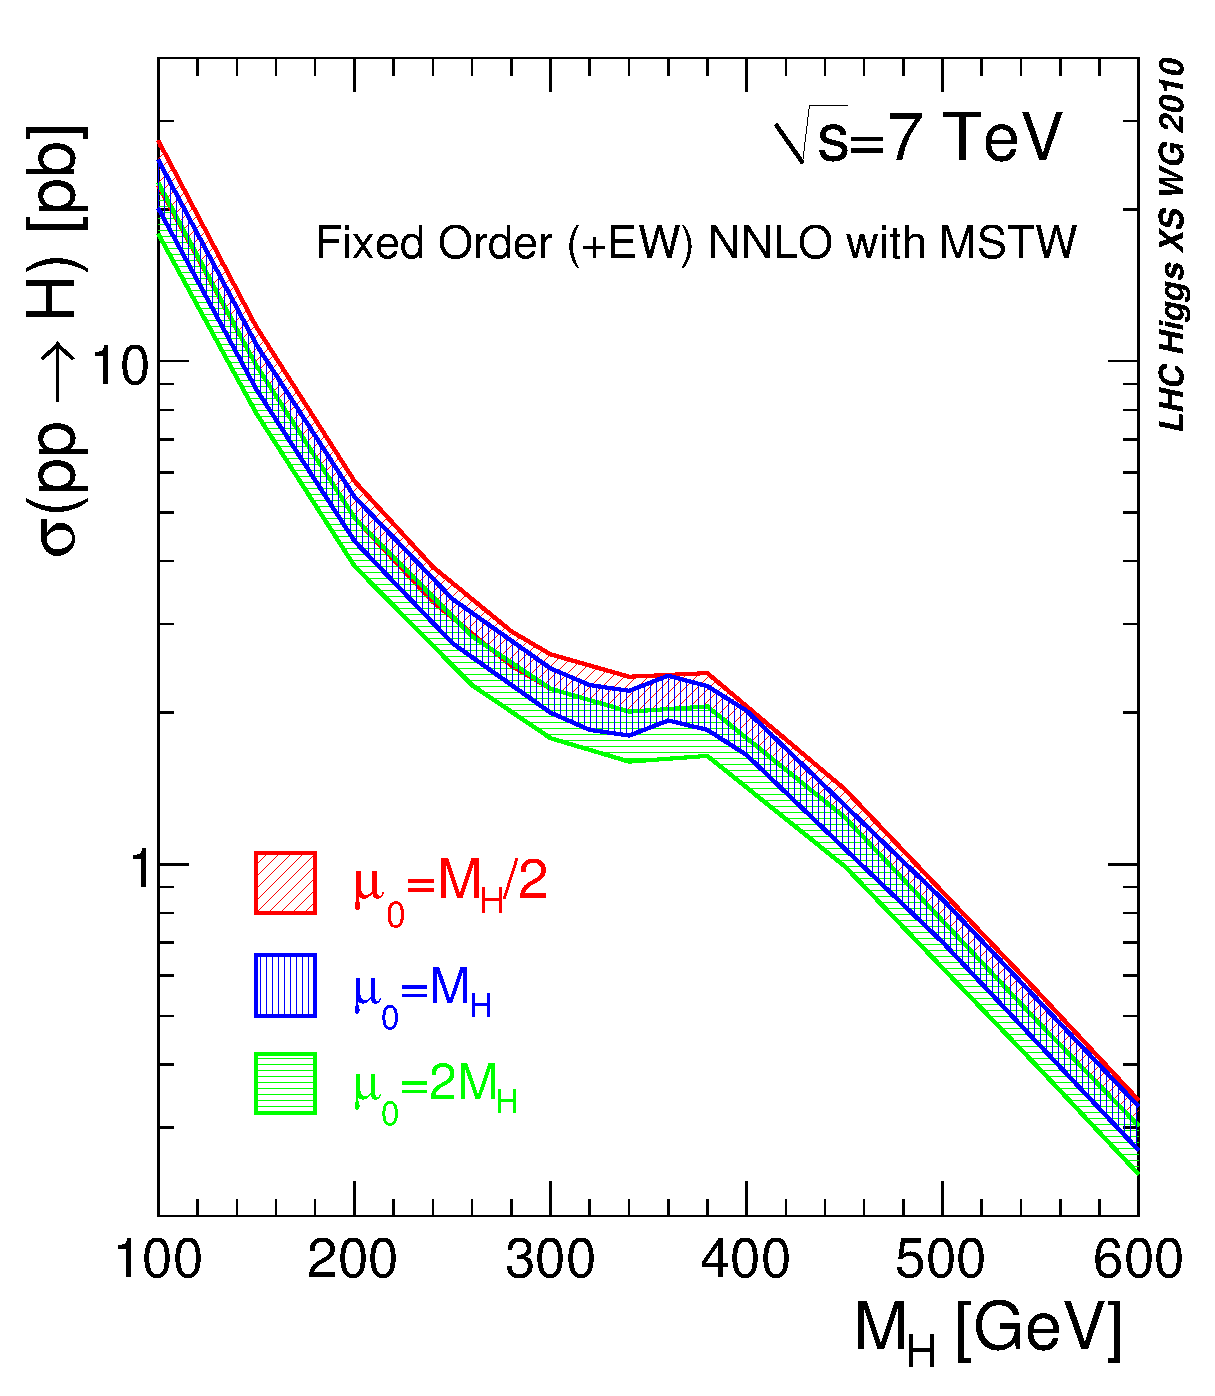
\includegraphics[width=.42\linewidth]{YRHXS_ggF/YRHXS_ggF_fig3} &
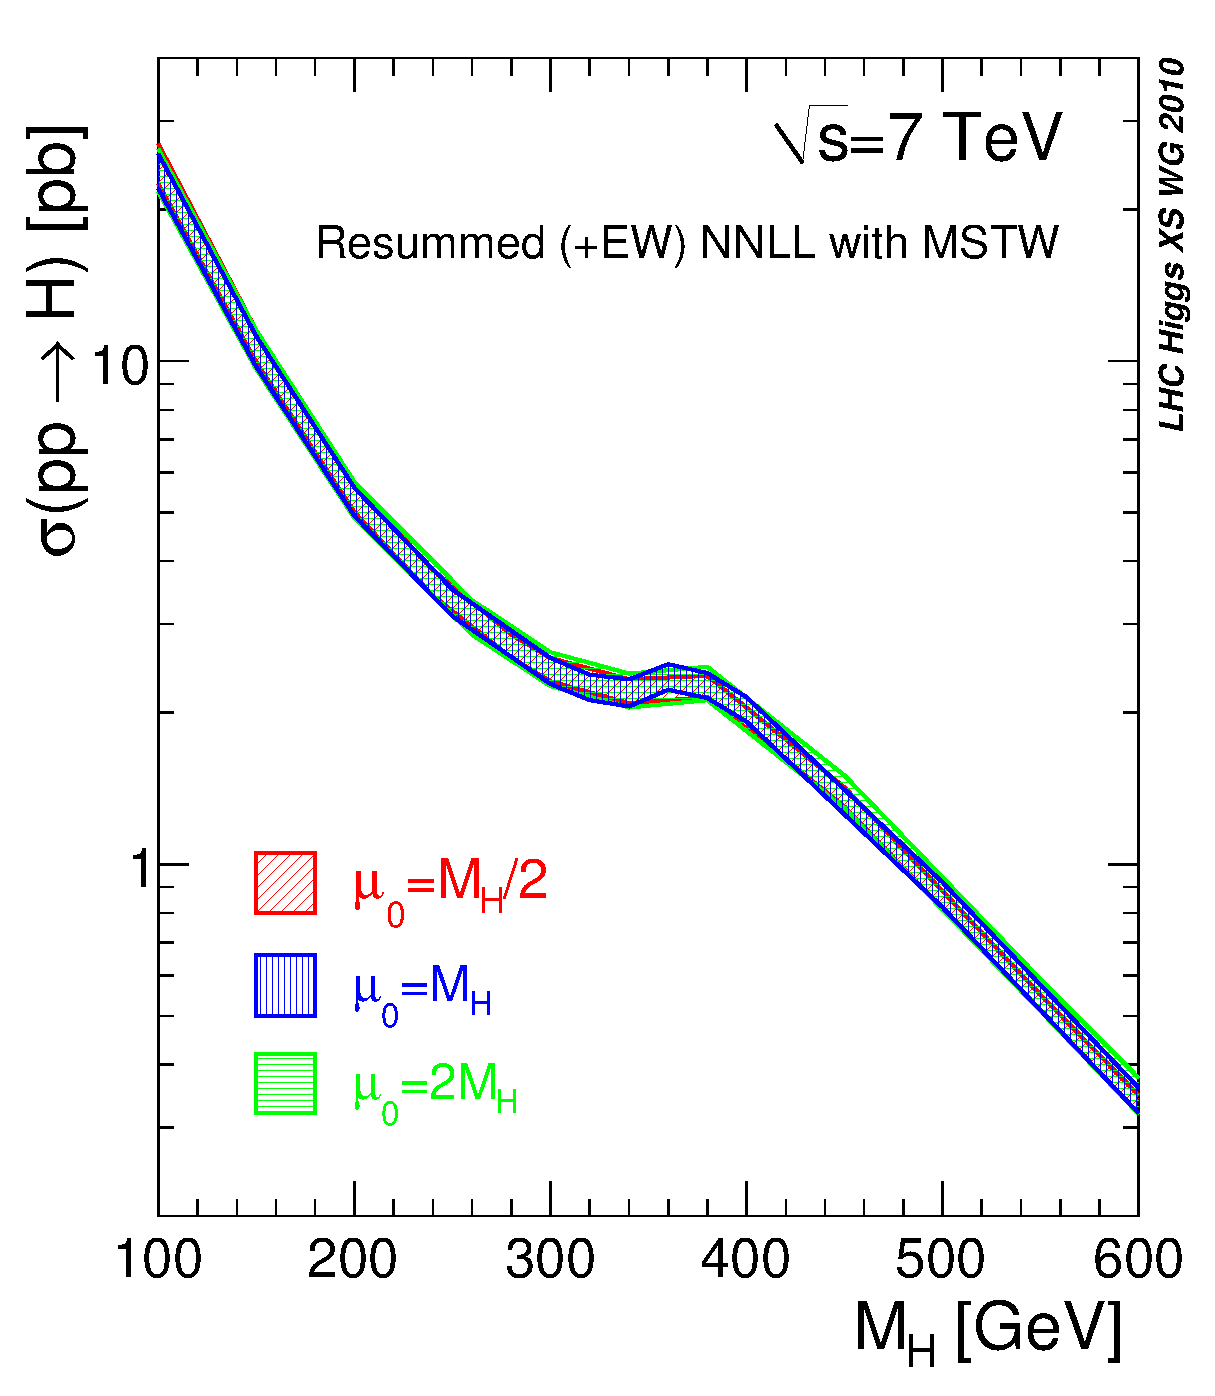
\includegraphics[width=.42\linewidth]{YRHXS_ggF/YRHXS_ggF_fig4} \\
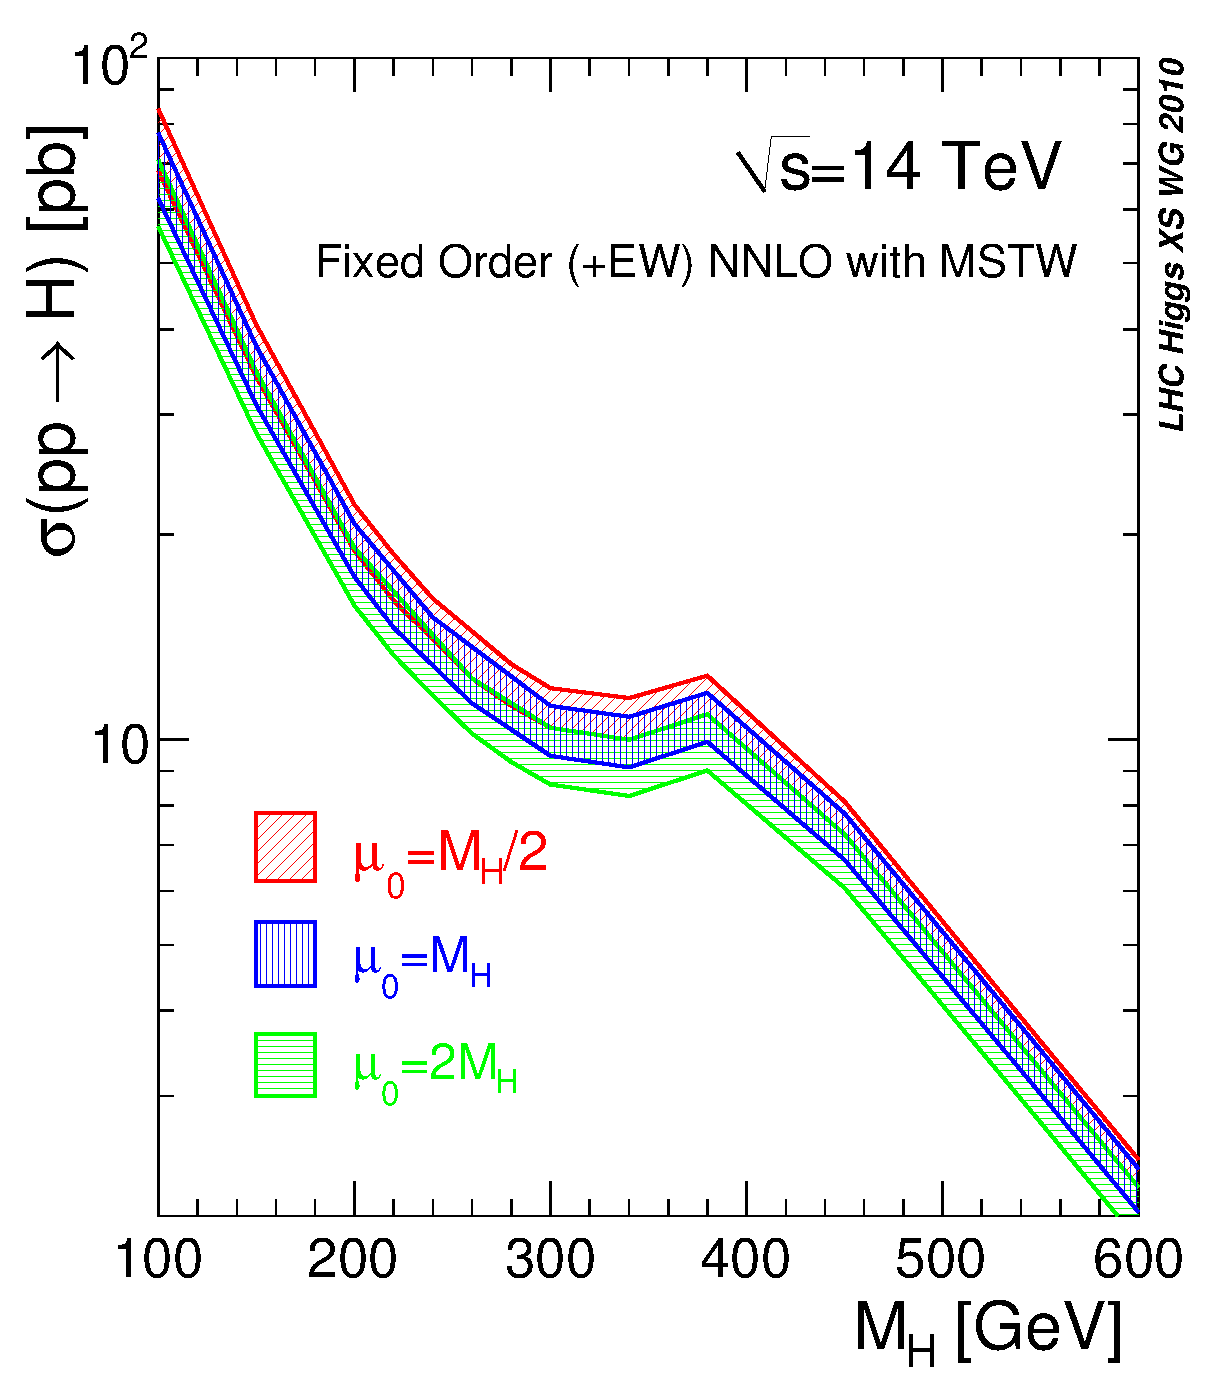
\includegraphics[width=.42\linewidth]{YRHXS_ggF/YRHXS_ggF_fig5} &
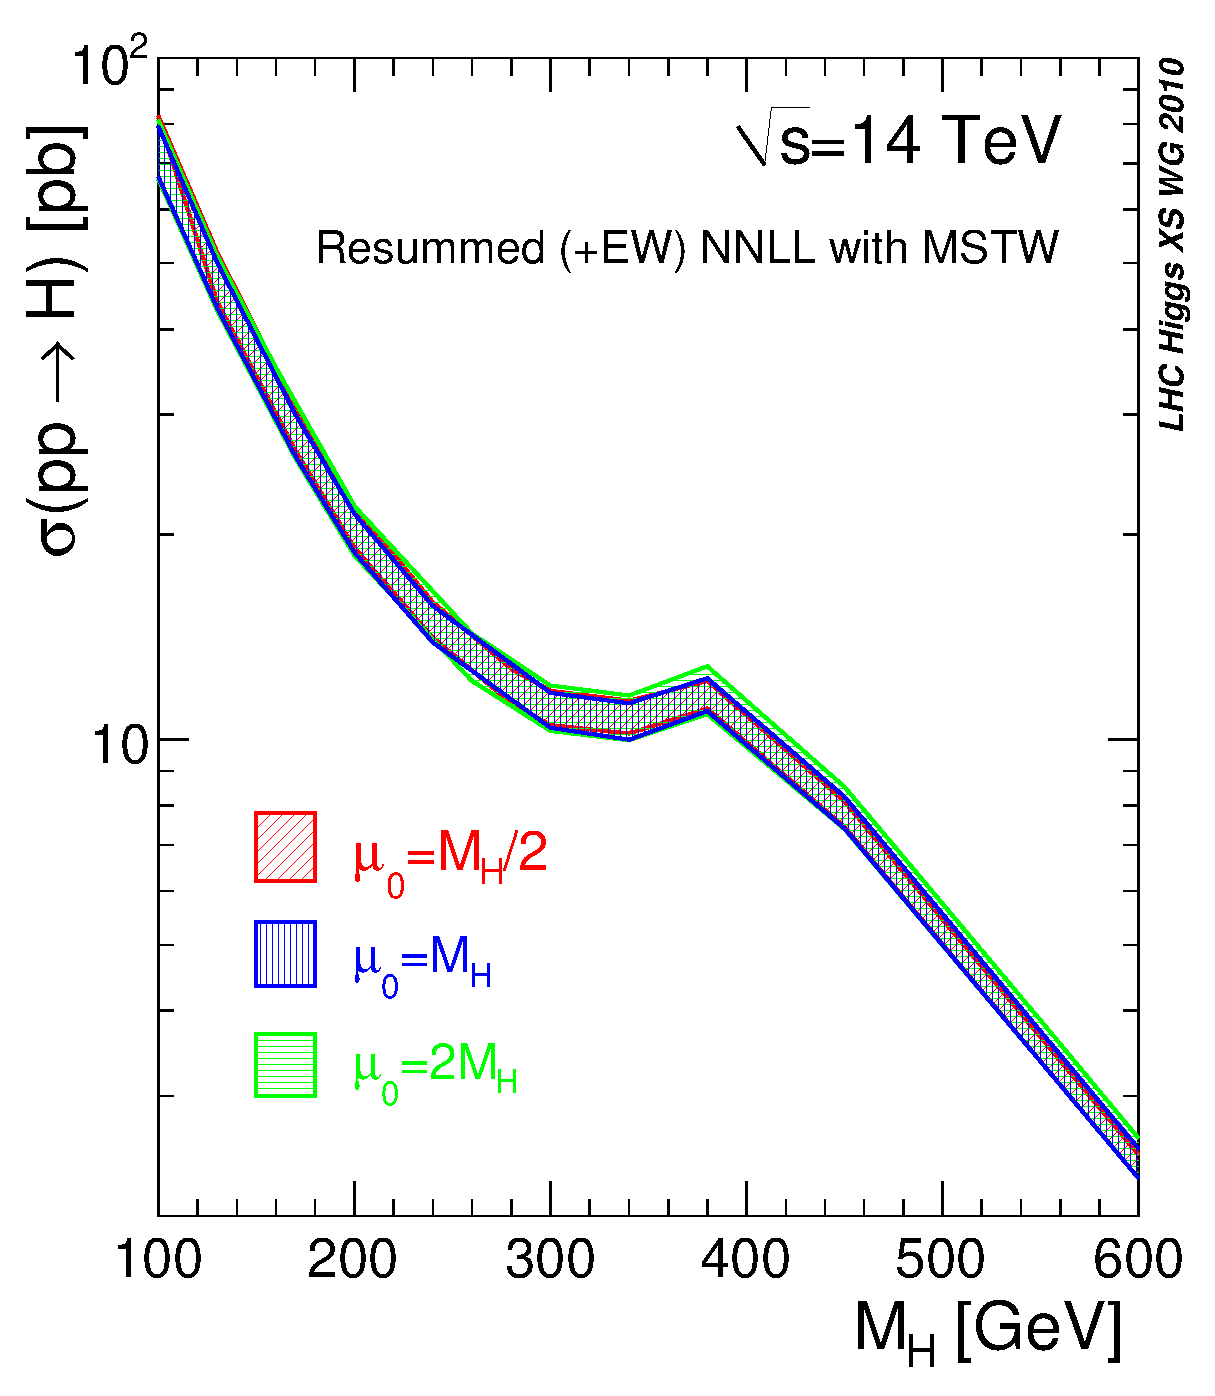
\includegraphics[width=.42\linewidth]{YRHXS_ggF/YRHXS_ggF_fig6} \\
\end{tabular}
\end{center}
\caption{Comparison of NNLO and NNLL bands with different choice of the central scale.}
\label{fig:compband}
\end{figure}




In principle, the uncertainty obtained through scale variations
can only give a lower limit on the {\it true} uncertainty.
Nonetheless, we point out that the results of ABPS and dFG are consistent with
those obtained at the previous order (i.e., dFG NNLL bands overlap with the NNLO band, and ABPS NNLO band overlap
with the NLO band), thus suggesting that the uncertainty obtained with this procedure provides a
reasonable estimate of the true perturbative uncertainty.  At $\sqrt{s}=7$ $(14)\UTeV$ the scale uncertainty of the ABPS result is about $\pm 9{-}10\%$ ($\pm 8{-}13\%$) in the range 
$\MH=100{-}300$\UGeV, and it decreases to about $\pm 7\%$ ($\pm 5\%$) as $\MH$ increases.
At $\sqrt{s}=7$ $(14)\UTeV$ the scale uncertainty of the dFG result is about $\pm 6{-}8\%$ ($\pm 6{-}9\%$) in the range $\MH=100{-}300$\UGeV, and it decreases slightly to about $\pm 5{-}7\%$ ($\pm 5\%$) as $\MH$ increases.

\item[$\bullet$] Another source of perturbative uncertainty on the partonic cross sections comes from the implementation of
the EW corrections. Both ABPS and dFG results are obtained in the complete factorization scheme discussed above.
The partial factorization scheme would lead to a change of the results ranging
from about $-3 \%$ ($\MH=110$\UGeV) to $+1\%$ ($\MH=300$\UGeV).  We note that the effective-theory calculation of \Bref{Anastasiou:2008tj} 
supports the use of the complete factorization scheme.  When the three-loop mixed QCD--EW correction derived there is normalized with the 
exact two-loop light-quark terms derived in \Brefs{Actis:2008ug,Actis:2008ts}, the dominant parts of the exact QCD corrections to 
the EW contributions are properly included.  This is the same reason that the NLO correction found using the large-$\Mt$ approximation 
only differs from the exact result by $10{-}15\%$ even for $\MH \sim 1$\UTeV, well outside the expected range of validity $\MH < 2 \Mt$. We expect that the 
exact three-loop mixed QCD--EW correction is estimated with a similar $\pm 10\%$ uncertainty using the effective-theory calculation of 
\Bref{Anastasiou:2008tj}.  As the two-loop EW contribution to the cross section reaches a 
maximum of only $+5\%$, we estimate an uncertainty of $\pm 1\%$ coming from missing EW corrections for $\MH \lsim 300$\UGeV.


\item[$\bullet$]  The use of the large-$\Mt$ approximation induces another source of uncertainty.
The ABPS and dFG calculations both include the exact NLO corrections with full dependence on the masses of the top and bottom quarks. 
The NNLO (NNLL) top-quark contributions are instead evaluated in the large-$\Mt$ limit. In \Brefs{Marzani:2008az,Harlander:2009bw,Harlander:2009mq,Harlander:2009my,Pak:2009bx,Pak:2009dg}
subleading corrections to the large-$\Mt$ limit have been computed. These
works have shown that for a relatively light Higgs boson ($\MH\lsim 300$\UGeV),
the approximation works to better than $1\%$. For a heavier Higgs boson
($\MH\gsim 300$\UGeV), the accuracy of the large-$\Mt$ approximation is expected to be worse, but still within a few percent.

\item[$\bullet$] Different choices of the input quark masses $\Mt$ and $\Mb$ lead to
a scheme dependence in the cross section.  We have 
checked that different values of $\Mt$ produce a negligible effect on the final cross section.  Although the contribution of the bottom quark to the 
production rate is much smaller than that of the top quark, large logarithms of the form ${\rm ln}(\MH / \Mb)$ lead to a non-negligible shift in the 
cross section. We estimate this by evaluating the cross section using both the pole mass and the $\MSbar$ mass for the \PQb\ quark, and interpreting 
the difference as a measure of uncertainty.  We use the $\MSbar$ mass evaluated at the renormalization scale, $\Mb(\mu_R)$. This leads to an uncertainty estimate of approximately $\pm 1{-}2\%$ on the final result.


\item[$\bullet$] The other important source of uncertainty in the cross section is
the one coming from PDFs.
Modern PDF sets let the user estimate the experimental uncertainty
originating from the accuracy of the data points used to perform the fit.
The MSTW2008 NNLO set \cite{Martin:2009iq} provides 40 different grids that allow evaluation of the experimental uncertainties according
to the procedure discussed in \Bref{Martin:2002aw}.
A related and important uncertainty is the one coming from the value of the QCD coupling.
Higgs production through gluon fusion starts at ${\cal O}(\alphas^2)$ and thus
this uncertainty is expected to have a sizeable effect on the production rate.  
Recently, the MSTW collaboration has studied the combined effect of PDF+$\alphas$
uncertainties~\cite{Martin:2009bu}.
The PDF+$\alphas$ uncertainties at $68\%$ confidence limit (CL) of the ABPS and dFG calculations are
reported in \Trefs{tab:dFG7}--\ref{tab:ABPS14}.
The uncertainties turn out to be quite similar,
being about $\pm 3{-}4\%$ in the range $\MH=100{-}300$\UGeV\ both at $\sqrt{s}=7\UTeV$ and $14$\UTeV. At $\sqrt{s}=7$ $(14)\UTeV$ they
increase to about $\pm 8{-}9\%$ ($\pm 5\%$) at high Higgs-boson masses.
In \Trefs{tab:dFG7}--\ref{tab:ABPS14} we also report the
uncertainties (see \refS{sec:pdf4lhcreco}) obtained through the PDF4LHC recommendation\footnote{We thank A. Vicini for providing us with the PDF4LHC correction factors.} \cite{PDF4LHCwebpage}.
At $7$ $(14)\UTeV$ the uncertainties are about $\pm 7{-}8\%$ ($\pm 6{-}7\%$) in the range $\MH=100{-}300$\UGeV,
and increase at high Higgs-boson masses. This is not completely unexpected: as the Higgs mass increases,
larger values of $x$ are probed, where the gluon distribution is more uncertain.

We finally point out that, besides MSTW, we have at present three other
NNLO parton analyses: ABKM09 \cite{Alekhin:2009ni}, JR09VFNNLO
\cite{JimenezDelgado:2009tv}, and HERAPDF \cite{CooperSarkar:2010ik}. These PDF sets tend to give smaller cross sections
both at $7\UTeV$ and $14\UTeV$ with respect to MSTW.
For example, at $14\UTeV$
the ABKM09 (JR09) result is smaller than the MSTW result by about $6{-}10\%$ ($13{-}8\%$)
in the range $\MH=100{-}300$\UGeV.
At $7\UTeV$ the ABKM09 (JR09) cross section is smaller than the MSTW cross section
by $9{-}16\%$ ($12{-}4\%$) in the same range of Higgs-boson masses.
HERAPDF has released two NNLO PDF sets corresponding to $\alphas(\MZ)=0.1145$ and $\alphas(\MZ)=0.1176$.
At $14\UTeV$ the result corresponding to $\alphas(\MZ)=0.1145$ ($\alphas(\MZ)=0.1176$)
is smaller than the MSTW result by about $8{-}10\%$ ($4{-}5\%$).
At $7\UTeV$ the cross section corresponding to $\alphas(\MZ)=0.1145$ ($\alphas(\MZ)=0.1176$)
is smaller than the MSTW result by about $10{-}14\%$ ($5{-}7\%$).


\end{itemize}

%\subsection{Other calculations: Baglio/Djouadi and Ahrens et al.}
%\subsection{Other calculations}
\subsection{Cross-section predictions II}
\label{se:ggfXS2}

\noindent
%Other groups have presented updated results for Higgs-boson cross sections.  We address here the features of each and comment on the differences between 
%these and the dFG and ABPS analyses presented above.

%%%%%%%%%%%%%%


	 A study of both the central value and uncertainty of Higgs production
cross sections at the Tevatron was performed in \Bref{Baglio:2010um}. We refer to this
analysis with the acronym BD. The BD study was later extended to cover LHC
production \cite{Baglio:2010ae}, and the results are reported in
\Trefs{tab:BD7} and \ref{tab:BD14}. BD use  a
fixed-order calculation with the exact top- and bottom-quark mass effects at
NLO, and then add on the NNLO top contributions in the large-$m_t$ limit as well
as the electroweak corrections at NLO and NNLO, as done in ABPS. They assume a
central scale value $\mu_0=  \MH/2$, as also do ABPS. This leads to an
excellent agreement in central value and relatively good agreement in the
estimated scale variation error with the dFG and ABPS results. BD estimate the
error arising from the PDFs and $\alphas$ differently than do dFG and ABPS.
They first choose to consider the 90\%\ CL PDF+$\Delta^{\rm exp}\alphas$
uncertainty and then define an additional theoretical error of $\Delta^{\rm
th}\alphas = 0.002$ on the strong coupling constant and use PDF grids with a
fixed $\alphas$ provided by MSTW to define a resulting uncertainty on the
production cross section. The resulting BD uncertainty is then added in quadrature
with the combined PDF+$\Delta^{\rm exp}\alphas$  uncertainty (at 90\%\ CL)
obtained by using the MSTW procedure ~\cite{Martin:2009bu}, giving a combined PDF+$\Delta^{\rm 
exp+th}\alphas$ uncertainty estimate of $\pm 10\%$ for Higgs masses below 350
GeV. The BD procedure is motivated by having the PDF+$\alphas$ uncertainty
bands obtained using MSTW to be consistent with those obtained with the PDF set
of \Bref{Alekhin:2009ni}. The ensuing BD uncertainty is only slightly larger than the one
obtained by following the PDF4LHC recommendation. BD finally combine the
uncertainties as follows: the PDF+$\alphas$ uncertainties are evaluated
directly on the maximum and minimum cross sections that arise from scale
variation. This gives a combined BD uncertainty that is comparable to that obtained
with a linear sum of the scale and PDF+$\alphas$ uncertainties. 

The major difference between the BD estimate for the theory uncertainty compared
to dFG and ABPS, is that an additional uncertainty, which is mainly due to the
use of the effective-field-theory approach beyond NLO,  is considered. It
consists of three main components: $i)$ the difference between the partial and
complete factorisation schemes in the NLO electroweak 
corrections~\cite{Actis:2008ug} which
approximately is equivalent to the contributions of the mixed NNLO
QCD--electroweak corrections obtained in the limit  $\MH\muchless \MW$~\cite{Anastasiou:2008tj}; $ii)$ 
the missing \PQb-quark loop contribution at NNLO (and its interference with the
top-quark loop) and the scheme dependence in the renormalisation of the
\PQb-quark mass in the NLO QCD contributions; $iii)$ the use of the $\Mt \to
\infty$ effective approximation  for Higgs masses beyond the $2\Mt$ threshold in
the NNLO QCD contribution. The (linear) sum of these three uncertainties turns
out to be quite large: it is at the  level of about $6{-}7\%$ in the mass range
$\MH \lsim 160\UGeV$ where the  difference between the partial and complete
factorisation approaches is significant and becomes even larger for $\MH\!
\gsim 600\UGeV$ where the $\Mt \to \infty$ approximation starts to fail
badly. 

When the EFT uncertainty is added linearly with the combined scale and
PDF+$\alphas$ uncertainty, the total BD theoretical uncertainties
become definitely large, being at $\sqrt s=7$ TeV, about $\pm 25{-}30\%$
in the low- and high-Higgs mass  ranges.

\begin{table}[!h]

%{\small%
%\let\lbr\{\def\{{\char'173}%
%\let\rbr\}\def\}{\char'175}%
%\renewcommand{\arraystretch}{0.9}
%\vspace*{-1mm}

%\thisfloatpagestyle{empty}
%   \vspace{-\headsep}
   \begin{center}
   \ccaption{}{\label{tab:BD7}{Results on $\Pp\Pp(\Pg\Pg)\to \PH+X$ cross
    sections with $\sqrt{s}=7$\UTeV\ based on BD calculation with MSTW
    PDFs.}}
    \small
    \begin{tabular}{cccccc}\hline
    $\MH[\UGeVZ]$ & $\sigma[\UpbZ]$  & Scale [\%] &  PDF+$\Delta^{exp+th}_{\alphas}$  [\%]  & ${\rm EFT}$  [\%]  \\ \hline
$90$  & $29.79$ & ${+10.4 \; -12.1}$ & ${+9.3}\;{ -8.9}$ & ${\pm 7.8} $  \\
$95$  & $26.77$ & ${+10.1 \; -11. }$ & ${+9.2}\;{ -8.9}$ & ${\pm 7.7} $  \\  
$100$ & $24.25$ & ${+9.9 \; -10.7 }$ & ${+9.2}\;{ -8.8}$ & ${\pm 7.6} $  \\  
$105$ & $22.01$ & ${+9.6 \; -10.5 }$ & ${+9.2}\;{ -8.8}$ & ${\pm 7.5} $  \\  
$110$ & $20.06$ & ${+9.4 \; -10.3 }$ & ${+9.1}\;{ -8.8}$ & ${\pm 7.4} $  \\  
$115$ & $18.35$ & ${+9.1 \; -10.2 }$ & ${+9.1}\;{ -8.8}$ & ${\pm 7.3} $  \\  
$120$ & $16.84$ & ${+8.9 \; -10.2 }$ & ${+9.1}\;{ -8.8}$ & ${\pm 7.3} $  \\  
$125$ & $15.51$ & ${ +8.8 \; -9.9 }$ & ${+9.1}\;{ -8.8}$ & ${\pm 7.2} $  \\  
$130$ & $14.32$ & ${ +8.5 \; -9.8 }$ & ${+9.1}\;{ -8.8}$ & ${\pm 7.1} $  \\  
$135$ & $13.26$ & ${ +8.4 \; -9.6 }$ & ${+9.1}\;{ -8.8}$ & ${\pm 7.0} $  \\  
$140$ & $12.31$ & ${ +8.3 \; -9.5 }$ & ${+9.1}\;{ -8.8}$ & ${\pm 7.0} $  \\  
$145$ & $11.45$ & ${ +8.2 \; -9.5 }$ & ${+9.1}\;{ -8.8}$ & ${\pm 6.9} $  \\  
$150$ & $10.67$ & ${ +8.1 \; -9.5 }$ & ${+9.1}\;{ -8.8}$ & ${\pm 6.8} $  \\  
$155$ & $9.94$  & ${ +7.9 \; -9.4 }$ & ${+9.1}\;{ -8.8}$ & ${\pm 6.6} $  \\  
$160$ & $9.21$  & ${ +7.8 \; -9.4 }$ & ${+9.1}\;{ -8.8}$ & ${\pm 5.9} $  \\  
$165$ & $8.47$  & ${ +7.7 \; -9.4 }$ & ${+9.1}\;{ -8.8}$ & ${\pm 4.9} $  \\  
$170$ & $7.87$  & ${ +7.7 \; -9.4 }$ & ${+9.1}\;{ -8.8}$ & ${\pm 4.2} $  \\  
$175$ & $7.35$  & ${ +7.6 \; -9.4 }$ & ${+9.1}\;{ -8.9}$ & ${\pm 3.7} $  \\  
$180$ & $6.86$  & ${ +7.5 \; -9.3 }$ & ${+9.2}\;{ -8.9}$ & ${\pm 3.1} $  \\  
$185$ & $6.42$  & ${ +7.4 \; -9.3 }$ & ${+9.2}\;{ -8.9}$ & ${\pm 3.0} $  \\  
$190$ & $6.01$  & ${ +7.4 \; -9.3 }$ & ${+9.2}\;{ -8.9}$ & ${\pm 3.4} $  \\  
$195$ & $5.65$  & ${ +7.4 \; -9.3 }$ & ${+9.2}\;{ -8.9}$ & ${\pm 3.6} $  \\  
$200$ & $5.34$  & ${ +7.3 \; -9.3 }$ & ${+9.3}\;{ -9.0}$ & ${\pm 3.7} $  \\  
$210$ & $4.81$  & ${ +7.2 \; -9.3 }$ & ${+9.3}\;{ -9.0}$ & ${\pm 3.7} $  \\  
$220$ & $4.36$  & ${ +7.2 \; -9.2 }$ & ${+9.3}\;{ -9.1}$ & ${\pm 3.6} $  \\  
$230$ & $3.97$  & ${ +7.0 \; -9.2 }$ & ${+9.4}\;{ -9.2}$ & ${\pm 3.5} $  \\  
$240$ & $3.65$  & ${ +7.0 \; -9.2 }$ & ${+9.5}\;{ -9.2}$ & ${\pm 3.3} $  \\  
$250$ & $3.37$  & ${ +6.9 \; -9.2 }$ & ${+9.5}\;{ -9.3}$ & ${\pm 3.1} $  \\  
$260$ & $3.11$  & ${ +6.8 \; -9.2 }$ & ${+9.6}\;{ -9.4}$ & ${\pm 3.0} $  \\  
$270$ & $2.89$  & ${ +6.7 \; -9.2 }$ & ${+9.7}\;{ -9.5}$ & ${\pm 2.8} $  \\  
$280$ & $2.71$  & ${ +6.8 \; -9.2 }$ & ${+9.8}\;{ -9.5}$ & ${\pm 2.6} $  \\  
$290$ & $2.55$  & ${ +6.8 \; -9.1 }$ & ${+9.8}\;{ -9.6}$ & ${\pm 2.4} $  \\  
$300$ & $2.42$  & ${ +6.7 \; -9.1 }$ & ${+9.9}\;{ -9.7}$ & ${\pm 2.3} $  \\  
$320$ & $2.23$  & ${ +6.7 \; -9.2 }$ & ${+10.1}\;{-9.9}$ & ${\pm 2.3} $  \\  
$340$ & $2.19$  & ${ +6.9 \; -9.2 }$ & ${+10.3}\;{-10.1}$& ${\pm 3.0} $ \\  
$360$ & $2.31$  & ${ +7.0 \; -9.2 }$ & ${+10.5}\;{-10.3}$& ${\pm 4.1} $ \\  
$380$ & $2.18$  & ${ +6.3 \; -9.1 }$ & ${+10.7}\;{-10.5}$& ${\pm 2.5} $  \\  
$400$ & $1.93$  & ${ +5.9 \; -8.8 }$ & ${+11.0}\;{-10.7}$& ${\pm 3.1} $  \\  
$450$ & $1.27$  & ${ +5.0 \; -8.4 }$ & ${+11.6}\;{-11.3}$& ${\pm 4.0} $  \\  
$500$ & $0.79$  & ${ +4.4 \; -8.1 }$ & ${+12.2}\;{-11.9}$& ${\pm 4.5} $  \\  
$550$ & $0.49$  & ${ +4.0 \; -7.9 }$ & ${+12.7}\;{-12.4}$& ${\pm 5.5} $  \\  
$600$ & $0.31$  & ${ +3.7 \; -7.7 }$ & ${+13.3}\;{-13.0}$& ${\pm 6.6} $  \\  
$650$ & $0.20$  & ${ +3.5 \; -7.6 }$ & ${+14.0}\;{-13.5}$& ${\pm 7.5} $  \\  
$700$ & $0.13$  & ${ +3.4 \; -7.5 }$ & ${+14.7}\;{-14.1}$& ${\pm 8.3} $  \\  
$750$ & $0.08$  & ${ +3.3 \; -7.4 }$ & ${+15.4}\;{-14.6}$& ${\pm 9.0} $  \\  
$800$ & $0.06$  & ${ +3.1 \; -7.4 }$ & ${+16.2}\;{-15.1}$& ${\pm 9.7} $  \\  
$850$ & $0.04$  & ${ +3.1 \; -7.3 }$ & ${+17.1}\;{-15.7}$& ${\pm 10.2}$  \\  
$900$ & $0.03$  & ${ +3.0 \; -7.3 }$ & ${+18.0}\;{-16.2}$& ${\pm 10.8}$  \\  
$950$ & $0.02$  & ${ +3.0 \; -7.3 }$ & ${+18.9}\;{-16.8}$& ${\pm 11.3}$  \\  
$1000$& $0.01$  & ${ +2.9 \; -7.2 }$ & ${+19.9}\;{-17.3}$& ${\pm 11.8}$  \\ \hline
\end{tabular} 
\end{center} 
\end{table}

\begin{table}[!h]
%{\small%
%\let\lbr\{\def\{{\char'173}%
%\let\rbr\}\def\}{\char'175}%
%\renewcommand{\arraystretch}{0.9}
%\vspace{-\headsep}
%\vspace*{-1mm}

%\thisfloatpagestyle{empty}
%   \vspace{-\headsep}
   \begin{center}
   \ccaption{}{\label{tab:BD14}{Results on $\Pp\Pp(\Pg\Pg)\to \PH+X$
    cross sections with $\sqrt{s}=14$\UTeV\ based on BD calculation with MSTW PDFs.}}
    \small
    \begin{tabular}{cccccc}\hline
    $\MH[\UGeVZ]$ & $\sigma[\UpbZ]$  & Scale [\%] &  PDF+$\Delta^{exp+th}_{\alphas}$  [\%]  & ${\rm EFT}$  [\%] \\ \hline
$90$  & $90.02$ & ${+10.8 \; -14.3}$ & ${ +9.1\; -8.9}$ & ${\pm 8.3} $  \\  
$95$  & $82.09$ & ${+10.4 \; -13.8}$ & ${ +9.0\; -8.8}$ & ${\pm 8.2} $  \\  
$100$ & $75.41$ & ${+10.2 \; -13.4}$ & ${ +8.9\; -8.7}$ & ${\pm 8.1} $  \\  
$105$ & $69.38$ & ${+9.9 \; -13.0 }$ & ${ +8.8\; -8.7}$ & ${\pm 8.0} $  \\  
$110$ & $64.07$ & ${+9.6 \; -12.6 }$ & ${ +8.7\; -8.6}$ & ${\pm 7.9} $  \\  
$115$ & $59.37$ & ${+9.4 \; -12.2 }$ & ${ +8.7\; -8.5}$ & ${\pm 7.8} $  \\  
$120$ & $55.20$ & ${+9.2 \; -11.9 }$ & ${ +8.6\; -8.4}$ & ${\pm 7.7} $  \\  
$125$ & $51.45$ & ${+9.0 \; -11.6 }$ & ${ +8.5\; -8.4}$ & ${\pm 7.6 } $  \\  
$130$ & $48.09$ & ${+8.9 \; -11.4 }$ & ${ +8.5\; -8.3}$ & ${\pm 7.5 } $  \\  
$135$ & $45.06$ & ${+8.7 \; -11.1 }$ & ${ +8.4\; -8.2}$ & ${\pm 7.5 } $  \\  
$140$ & $42.30$ & ${+8.5 \; -10.8 }$ & ${ +8.4\; -8.2}$ & ${\pm 7.4 } $  \\  
$145$ & $39.80$ & ${+8.4 \; -10.6 }$ & ${ +8.3\; -8.1}$ & ${\pm 7.3 } $ \\  
$150$ & $37.50$ & ${+8.3 \; -10.4 }$ & ${ +8.3\; -8.1}$ & ${\pm 7.2 } $  \\  
$155$ & $35.32$ & ${+8.1 \; -10.2 }$ & ${ +8.3\; -8.1}$ & ${\pm 7.0 } $ \\  
$160$ & $33.08$ & ${+8.0 \; -10.0 }$ & ${ +8.2\; -8.0}$ & ${\pm 6.3 } $  \\  
$165$ & $30.77$ & ${ +7.9 \; -9.8 }$ & ${ +8.2\; -8.0}$ & ${\pm 5.3 } $ \\  
$170$ & $28.89$ & ${ +7.8 \; -9.7 }$ & ${ +8.2\; -8.0}$ & ${\pm 4.5 } $  \\  
$175$ & $27.24$ & ${ +7.8 \; -9.5 }$ & ${ +8.2\; -7.9}$ & ${\pm 4.0 } $  \\  
$180$ & $25.71$ & ${ +7.7 \; -9.4 }$ & ${ +8.2\; -7.9}$ & ${\pm 3.5 } $  \\  
$185$ & $24.28$ & ${ +7.6 \; -9.1 }$ & ${ +8.1\; -7.9}$ & ${\pm 3.3 } $  \\  
$190$ & $22.97$ & ${ +7.6 \; -9.1 }$ & ${ +8.1\; -7.9}$ & ${\pm 3.8 } $ \\  
$195$ & $21.83$ & ${ +7.5 \; -9.0 }$ & ${ +8.1\; -7.9}$ & ${\pm 4.0 } $ \\  
$200$ & $20.83$ & ${ +7.4 \; -8.8 }$ & ${ +8.1\; -7.9}$ & ${\pm 4.1 } $ \\  
$210$ & $19.10$ & ${ +7.3 \; -8.6 }$ & ${ +8.1\; -7.8}$ & ${\pm 4.1 } $  \\  
$220$ & $17.64$ & ${ +7.2 \; -8.4 }$ & ${ +8.1\; -7.8}$ & ${\pm 4.0 } $  \\  
$230$ & $16.38$ & ${ +7.1 \; -8.3 }$ & ${ +8.0\; -7.8}$ & ${\pm 3.8 } $ \\  
$240$ & $15.30$ & ${ +7.0 \; -8.2 }$ & ${ +8.0\; -7.8}$ & ${\pm 3.7 } $  \\  
$250$ & $14.38$ & ${ +6.9 \; -8.2 }$ & ${ +8.0\; -7.8}$ & ${\pm 3.5 } $  \\  
$260$ & $13.52$ & ${ +6.8 \; -8.1 }$ & ${ +8.0\; -7.8}$ & ${\pm 3.3 } $ \\  
$270$ & $12.79$ & ${ +6.7 \; -8.1 }$ & ${ +8.0\; -7.8}$ & ${\pm 3.1 } $  \\  
$280$ & $12.17$ & ${ +6.7 \; -8.1 }$ & ${ +8.0\; -7.8}$ & ${\pm 2.9 } $ \\  
$290$ & $11.65$ & ${ +6.6 \; -8.0 }$ & ${ +8.0\; -7.8}$ & ${\pm 2.8 } $  \\  
$300$ & $11.22$ & ${ +6.5 \; -8.0 }$ & ${ +8.0\; -7.8}$ & ${\pm 3.4 } $  \\  
$320$ & $10.70$ & ${ +6.5 \; -8.0 }$ & ${ +8.1\; -7.9}$ & ${\pm 3.1 } $ \\  
$340$ & $10.83$ & ${ +6.5 \; -8.0 }$ & ${ +8.1\; -7.9}$ & ${\pm 2.8 } $ \\  
$360$ & $11.77$ & ${ +6.4 \; -8.0 }$ & ${ +8.1\; -8.0}$ & ${\pm 3.5 } $  \\  
$380$ & $11.46$ & ${ +6.0 \; -7.7 }$ & ${ +8.2\; -8.1}$ & ${\pm 4.4 } $ \\  
$400$ & $10.46$ & ${ +5.6 \; -7.4 }$ & ${ +8.2\; -8.1}$ & ${\pm 5.0 } $ \\  
$450$ & $7.42$  & ${ +5.0 \; -7.0 }$ & ${ +8.4\; -8.3}$ & ${\pm 6.0 } $  \\  
$500$ & $4.97$  & ${ +4.6 \; -6.7 }$ & ${ +8.6\; -8.6}$ & ${\pm 6.4 } $ \\  
$550$ & $3.32$  & ${ +4.3 \; -6.5 }$ & ${ +8.9\; -8.8}$ & ${\pm 7.4 } $ \\  
$600$ & $2.24$  & ${ +4.1 \; -6.3 }$ & ${ +9.2\; -9.1}$ & ${\pm 8.3 } $  \\  
$650$ & $1.53$  & ${ +3.9 \; -6.2 }$ & ${ +9.5\; -9.4}$ & ${\pm 9.0 } $  \\  
$700$ & $1.05$  & ${ +3.8 \; -6.1 }$ & ${ +9.8\; -9.6}$ & ${\pm 9.6 } $  \\  
$750$ & $0.74$  & ${ +3.6 \; -6.0 }$ & ${+10.1\; -9.9}$ & ${\pm 10.1 } $  \\  
$800$ & $0.52$  & ${ +3.5 \; -6.0 }$ & ${+10.4\;-10.2}$ & ${\pm 10.5 } $ \\  
$850$ & $0.38$  & ${ +3.5 \; -5.9 }$ & ${+10.7\;-10.5}$ & ${\pm 11.0 } $  \\  
$900$ & $0.27$  & ${ +3.4 \; -5.9 }$ & ${+11.0\;-10.7}$ & ${\pm 11.3 } $  \\  
$950$ & $0.20$  & ${ +3.3 \; -5.8 }$ & ${+11.3\;-11.0}$ & ${\pm 11.7 } $ \\  
$1000$ & $0.15$ & ${ +3.3 \; -5.8 }$ & ${+11.5\;-11.3}$ & ${\pm 12.0 } $  \\ \hline
\end{tabular} 
\end{center} 
\end{table}


\subsection{An alternative cross-section calculation based on an
effective field theory}

In \Bref{Ahrens:2010rs} updated predictions for Higgs-boson production at the Tevatron and the LHC were presented.
The results of \Bref{Ahrens:2010rs} are based on the work of \Brefs{Ahrens:2008qu,Ahrens:2008nc},
where a new calculation of the Higgs production cross section was presented.
This calculation supplements the NNLO result, obtained in the large-$\Mt$ approximation, 
with soft-gluon resummation done in the framework of an effective field theory (EFT) approach, and with the resummation of
some ``$\pi^2$-terms'' originating from the analytic continuation of the gluon form factor.  These additional terms are obtained 
in the EFT formalism by choosing an imaginary matching scale, and are included by the authors to improve the convergence of the perturbative series.  
The update of \Bref{Ahrens:2010rs} treats both top- and bottom-quark loops in the heavy-quark approximation, and includes EW corrections 
assuming complete factorization.  In the range $\MH=115{-}200$\UGeV\ the central values of \Bref{Ahrens:2010rs} are in good agreement with those of the 
ABPS and dFG calculations (for example, the difference with the dFG results is at $1{-}2\%$ level).  However, we note that the reliability of $\pi^2$ resummation 
has been questioned, and that there are puzzling differences between this approach and the standard soft-gluon resummation.  The effect of 
resummation in \Bref{Ahrens:2010rs} is driven by the $\pi^2$ terms; without them, the effect of resummation is much smaller than the one obtained using the 
standard approach~\cite{Ahrens:2008nc}.  The numerical agreement between central values therefore appears accidental.  
Soft-gluon resummations typically deal with logarithmically terms that are enhanced in some region of the phase space.
As an example, in the soft-gluon resummation of \Bref{Catani:2003zt} the logarithmic terms are $\log^n(1-z)$ where
$1-z=1-\MH^2/{\hat s}$ is the distance from the partonic threshold. These logarithmic terms can be precisely traced back and identified at each 
perturbative order. On the contrary, $\pi^2$ terms are just numbers, and there is no limit in which they can dominate. Moreover, only those 
$\pi^2$ terms coming from the analytic continuation of the gluon form factor can actually be controlled in this way.  Other $\pi^2$ terms are
present at each order in perturbation theory, and they can be obtained only through an explicit computation.
We add a final comment on the perturbative uncertainties quoted in the calculation of \Bref{Ahrens:2010rs}. The scale uncertainty of the 
results are of the order of $\pm 3\%$ or smaller.
This should be contrasted with the uncertainties of the ABPS and dFG calculations, which are a factor of $2{-}3$ larger. Since the calculation of 
\Bref{Ahrens:2010rs} does not contain new information beyond NNLO with respect to those of ABPS, dFG, and BD, we feel uncomfortable with such a 
small uncertainty and believe it is underestimated. For comparison, it should be noticed that the perturbative uncertainty of a full N$^3$LO
calculation, estimated through scale variations, would be of the order of about $\pm 5\%$~\cite{Moch:2005ky}.

\clearpage
